%!TEX root = ../../main.tex
\section{Protein Structure Results}
\label{sec:Protein Structure Results}

\subsection{Bovine pancreatic insulin}
\label{sub:Bovine pancreatic insulin}

\subsubsection{Scale and B factors}
\label{subs:Scale and B factors - insulin}
Data were collected on a crystal of bovine pancreatic insulin (crystal ID 0259) as described in chapter \ref{chap:Dose Decay Modelling}.
The atomic composition used to provide expected intensity values, was obtained from the insulin structure with PDB code 2BN3.
The B factors could then be calculated for each image and are shown in Figure~\ref{fig:B factors per image - insulin}.
It can be seen that there are a couple of points that may be regarded as outliers in Figure~\ref{fig:B factors per image before outlier removal - insulin}.
To remove the outliers, the mean and standard deviation of the B factors were calculated and any B factor that was more than two standard deviations from the mean was removed.
The resulting B factor distribution is plotted in Figure~\ref{fig:B factors per image after outlier removal - insulin}.
\begin{figure}
    \centering
    \begin{subfigure}[b]{1.0\textwidth}
            \centering
            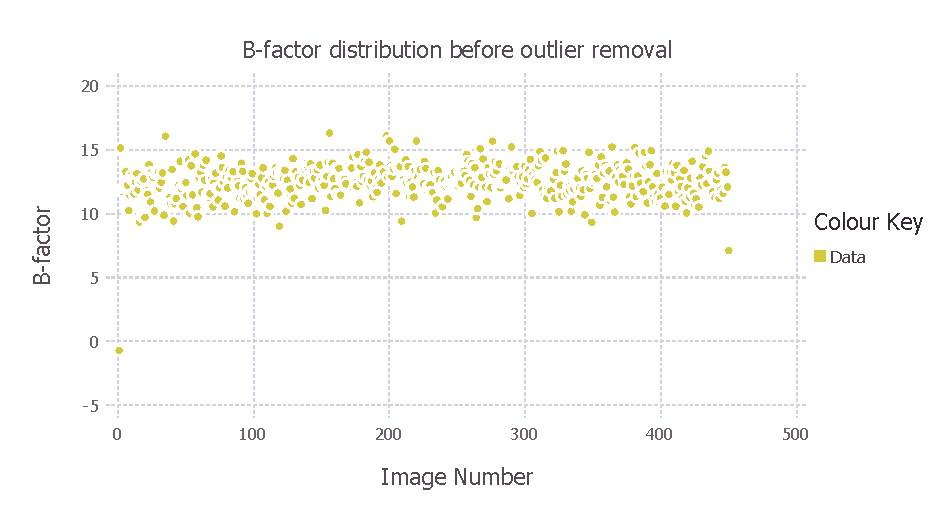
\includegraphics[width=\textwidth]{figures/datared/BFac_Plot_Before_outlier_removal.pdf}
            \caption{}
            \label{fig:B factors per image before outlier removal - insulin}
    \end{subfigure}
    \\
    \begin{subfigure}[b]{1.0\textwidth}
            \centering
            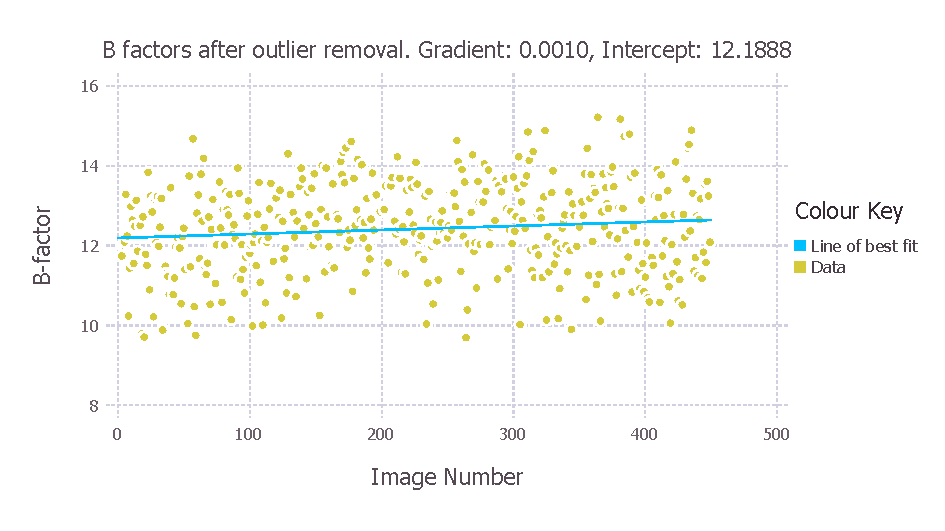
\includegraphics[width=\textwidth]{figures/datared/BFac_Plot_After_outlier_removal.pdf}
            \caption{}
            \label{fig:B factors per image after outlier removal - insulin}
    \end{subfigure}
    \caption{Calculated B factors for each image in the insulin dataset.
    (a) Distribution before outlier removal.
    (b) Distribution after outlier removal.
    The line of best fit (blue solid line) with gradient, $\Delta B$ = 0.001 and intercept = 12.189, is overlaid on the data.}
    \label{fig:B factors per image - insulin}
\end{figure}

To ensure that the B-factors exhibited linear behaviour, "damage corrected" B factors, $B_{dc}$, were calculated by rearranging the linear formula for the B factor increase.
\begin{equation}
    B^i_{dc} = B_i - \Delta B \times i,
\end{equation}
where $B_i$ is the B factor calculated at image $i$, and $\Delta B$ is the gradient of the line fitted to the data.
A histogram of the "damage corrected" B factor distribution was then plotted, which should be a Gaussian distribution centred on the intercept of the line in Figure~\ref{fig:B factors per image after outlier removal - insulin}.
Additionally a QQ plot was used to ensure that the data were normally distributed (Figure~\ref{fig:B factor QQ plot - insulin}).
The gradient $\Delta B$ was calculated to be 0.001$\,$\AA$^2$.
\begin{figure}
    \centering
    \begin{subfigure}[b]{1.0\textwidth}
            \centering
            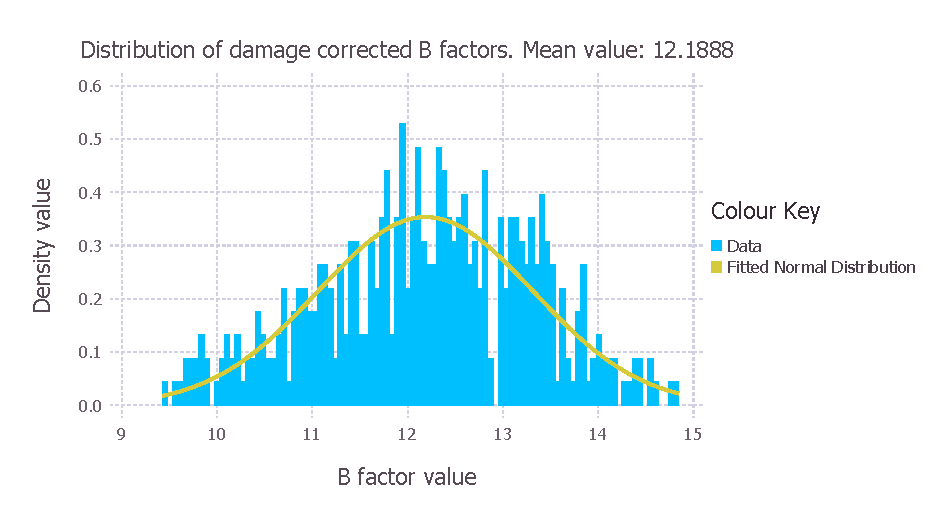
\includegraphics[width=\textwidth]{figures/datared/BFac_Distribution.pdf}
            \caption{}
            \label{fig:Damage corrected B factor distribution - insulin}
    \end{subfigure}
    \\
    \begin{subfigure}[b]{1.0\textwidth}
            \centering
            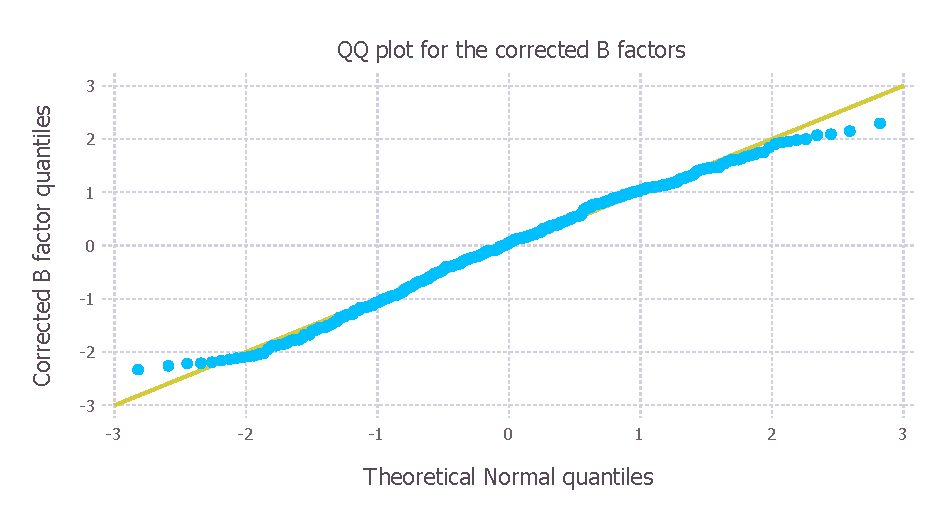
\includegraphics[width=\textwidth]{figures/datared/BFac_QQplot.pdf}
            \caption{Dose at which maximum curvature is reached}
            \label{fig:B factor QQ plot - insulin}
    \end{subfigure}
    \caption{(a) Histogram of damage corrected B factors.
    The Gaussian shape suggests that a linear assumption for the behaviour of B factors is suitable.
    (b) QQ plot for the damage corrected B factors.
    The linearity of the points prove that the distribution is actually Gaussian.}
    \label{fig:Gaussian B factor plots - insulin}
\end{figure}

The calculated scale factors are shown in Figure~\ref{fig:Scale factors per image - insulin}.
There did not appear to be any outliers by visual inspection (Figure~\ref{fig:Scale factors per image before outlier removal - insulin}), so there was no outlier rejected method performed for the scale factors.
The scale factors that corresponded to images that were removed from the B factor outlier rejection analysis were also omitted for consistency.
The resulting scale factors are shown in Figure~\ref{fig:Scale factors per image after outlier removal - insulin}.
\begin{figure}
    \centering
    \begin{subfigure}[b]{1.0\textwidth}
            \centering
            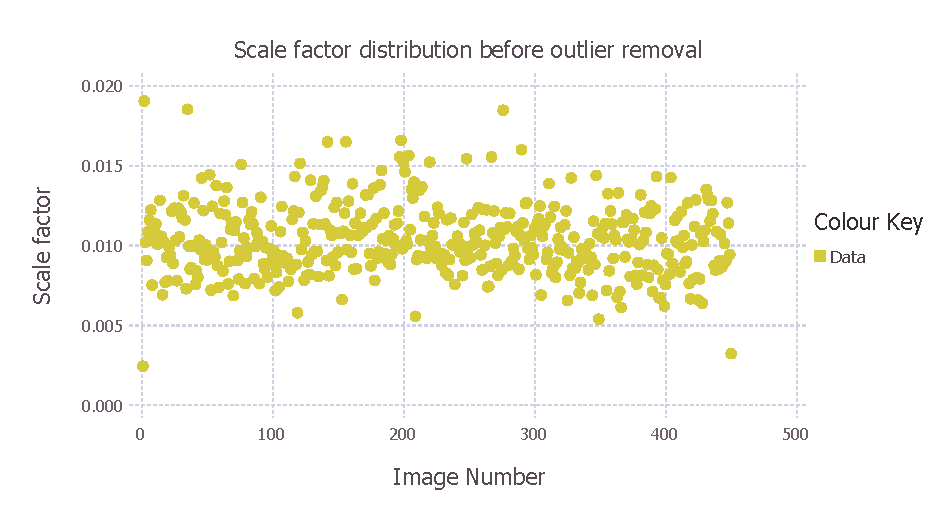
\includegraphics[width=\textwidth]{figures/datared/ScaleFac_Plot_Before_outlier_removal.pdf}
            \caption{}
            \label{fig:Scale factors per image before outlier removal - insulin}
    \end{subfigure}
    \\
    \begin{subfigure}[b]{1.0\textwidth}
            \centering
            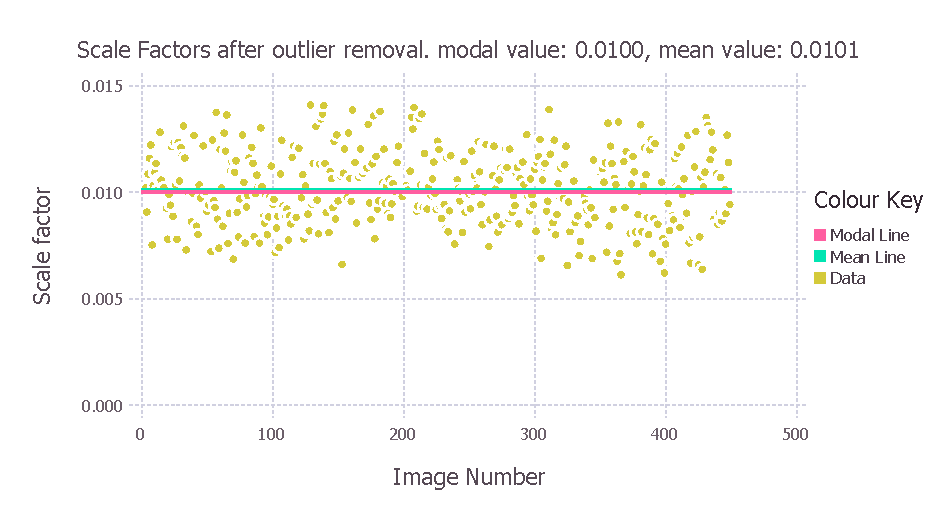
\includegraphics[width=\textwidth]{figures/datared/ScaleFac_Plot_After_outlier_removal.pdf}
            \caption{Dose at which maximum curvature is reached}
            \label{fig:Scale factors per image after outlier removal - insulin}
    \end{subfigure}
    \caption{Calculated scale factors for each image in the insulin dataset.
    (a) Distribution before outlier removal.
    (b) Distribution after outlier removal.
    The solid turquoise and solid pink lines represent the mean and mode of the distribution respectively.
    The fact that the mean and mode are close in value suggest that the distribution is Gaussian.}
    \label{fig:Scale factors per image - insulin}
\end{figure}

The distribution of scale factors shown as a histogram is shown in Figure~\ref{fig:Scale factor distribution after outlier removal - insulin}.
The fact that the mode and mean are very similar in value also suggests that the scale factor distribution is Gaussian.
However there is no guarantee that the scale factor distribution for a general experiment will be Gaussian and hence there are no checks for normality written for the scale factors.
In the forward-backward algorithm the scale factor is assumed constant.
Although this assumption is not true in the general case, it should be suitable for the diffraction experiment concerned where the insulin crystal is completely immersed in a tophat beam for a 45$^{\circ}$ rotation.
The mean value of 0.010 was used for the scale factor in the forward-backward algorithm.
\begin{figure}[ht!]
    \centering
    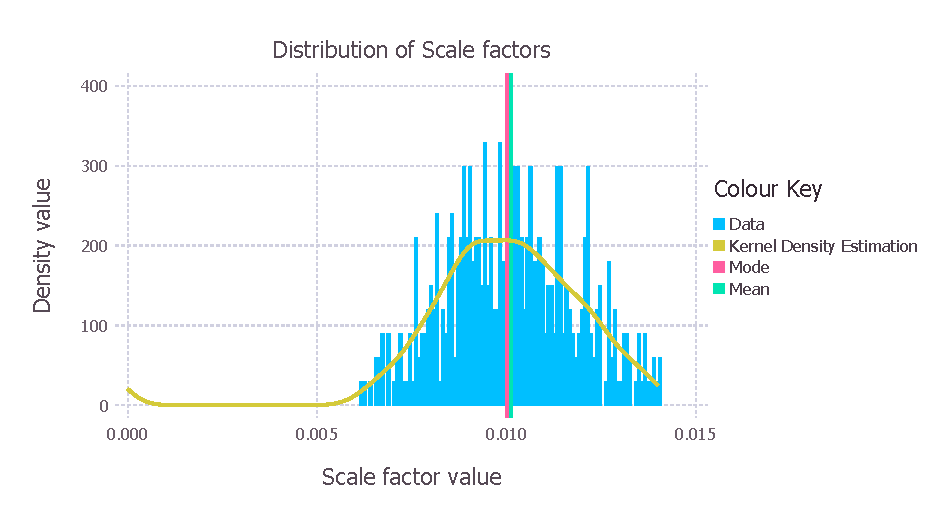
\includegraphics[width=1.0\textwidth]{figures/datared/ScaleFac_Distribution.pdf}
    \caption{Histogram of scale factors with the mean (solid turquoise line), mode (solid pink line) and kernel density estimation (solid gold line) overlaid.}
    \label{fig:Scale factor distribution after outlier removal - insulin}
\end{figure}

\subsubsection{Forward-backward algorithm}
\label{subs:Forward-backward algorithm - insulin}
The forward-backward algorithm was carried out with the following parameters defined:
\begin{itemize}
    \item the minimum and maximum number of forward-backward cycles for an individual reflection was 5 and 200 respectively.
    \item the forward-backward cycles was regarded to have converged if:
    \begin{enumerate}
        \item the maximum number of cycles had been reached (200)
        \item the absolute change in log likelihood between consecutive cycles was less than 0.1
        \item the change in initial amplitude value between consecutive cycles was less than 1
    \end{enumerate}
    \item reflections for which the Rician distribution was used for the amplitude process function were defined as reflections where $F_0/\sigma(F_0) <$ 3, where $F_0$ is the initial amplitude estimate.
\end{itemize}
Amplitude estimates resulting from applying the forward-backward algorithm for 4 reflections are shown in Figure~\ref{fig:Amplitude estimates - insulin}.
It can be seen for these reflections that the initial amplitude value estimated using CTRUNCATE is within the 95\% confidence region as estimated by the forward-backward algorithm.
This suggests that the constant scale factor assumption used for the simple scaling procedure used for this study is valid for this experiment.

Figures~\ref{fig:Amplitude estimates ref 0,30,38 - insulin} and \ref{fig:Amplitude estimates ref 0,37,11 - insulin} exhibit expected behaviour of the average refection since both of these reflections decay relatively smoothly as exposure time increases.
Figure~\ref{fig:Amplitude estimates ref 0,49,27 - insulin} shows a reflection whose amplitude increases as the exposure increases.
This demonstrates that the forward-backward algorithm is capable of capturing the different behaviours of various reflections despite the process function describing a monotonic decay of the amplitudes.

Figure~\ref{fig:Amplitude estimates ref 2,10,22 - insulin} shows a reflection where the behaviour is very irregular and not very smooth.
In this case it is very likely not to be caused by a physical phenomenon and is probably due to incorrect scaling of the data.
To prevent this problem, restraints should be imposed during the scaling procedure in a similar manner to those of existing scaling methods to ensure sufficient smoothness of reflection amplitudes\cite{evans2013,kabsch2010integration}.
It should be noted that not all sharp changes in amplitudes relate to noise/incorrect processing.
Mechanical or chemical changes of the structure can occur within a few seconds \cite{allan2012}.

Another detrimental feature of the forward-backward algorithm is the fact that the initial amplitude estimate is solely influenced by the amplitude estimate at the point where the observation is made.
This effect is prominent in Figures~\ref{fig:Amplitude estimates ref 0,37,11 - insulin} and \ref{fig:Amplitude estimates ref 0,49,27 - insulin}.
Therefore the initial amplitude estimate is not influenced by the multiplicity and hence erroneous estimates are more likely to arise if the first observation of a reflection is an outlier.
This can be overcome performing the forward-backward algorithm on each observation separately and merging the entire amplitude curves for equivalent reflections.
The relative uncertainties at each point in the data collection experiment will be different because the observations will be observed at different times.
This should ensure that the (possibly non-linear) behaviour of the reflection should still be captured by this method.
\begin{figure}
	\centering
    \begin{subfigure}[b]{1.0\textwidth}
        \centering
        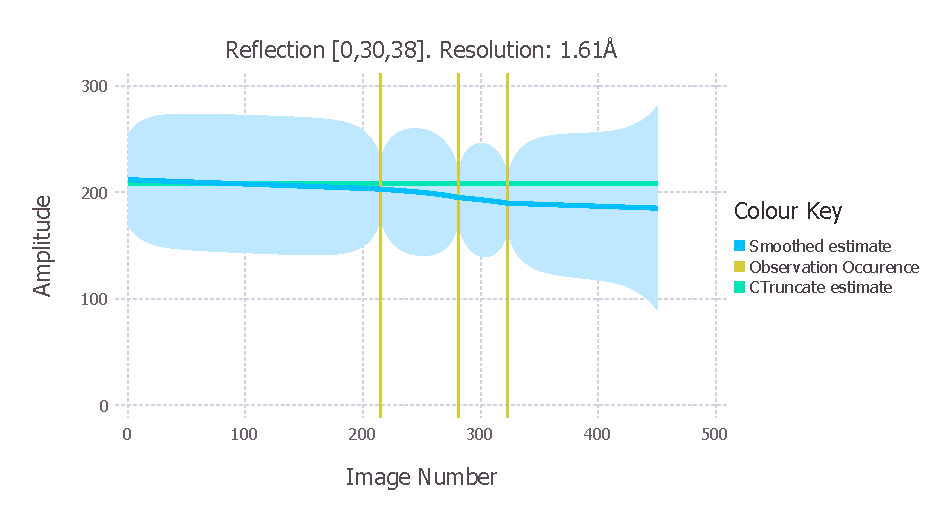
\includegraphics[width=\textwidth]{figures/datared/SmoothedPlot_0,30,38_res2.pdf}
        \caption{}
        \label{fig:Amplitude estimates ref 0,30,38 - insulin}
    \end{subfigure}
    \\
	\begin{subfigure}[b]{1.0\textwidth}
        \centering
        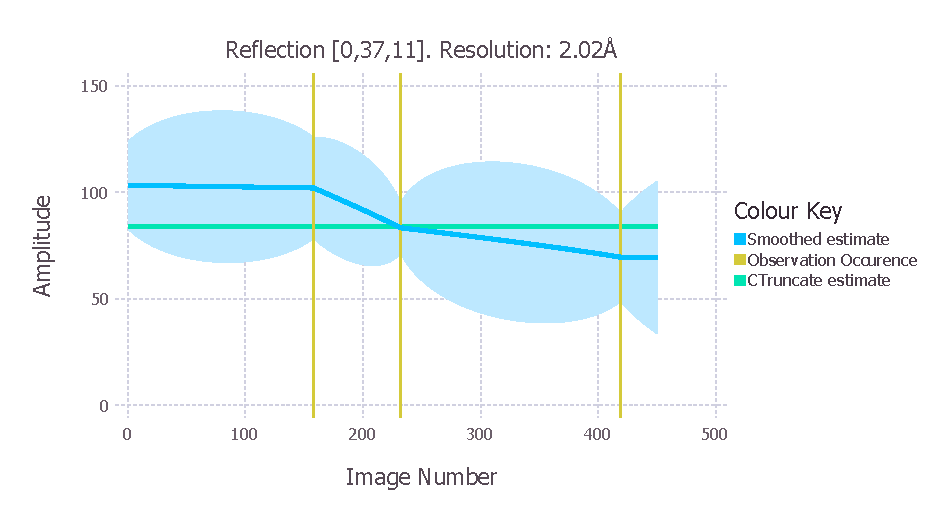
\includegraphics[width=\textwidth]{figures/datared/SmoothedPlot_0,37,11_res2.pdf}
        \caption{}
        \label{fig:Amplitude estimates ref 0,37,11 - insulin}
    \end{subfigure}
\end{figure}
\begin{figure}
    \ContinuedFloat
    \begin{subfigure}[b]{1.0\textwidth}
        \centering
        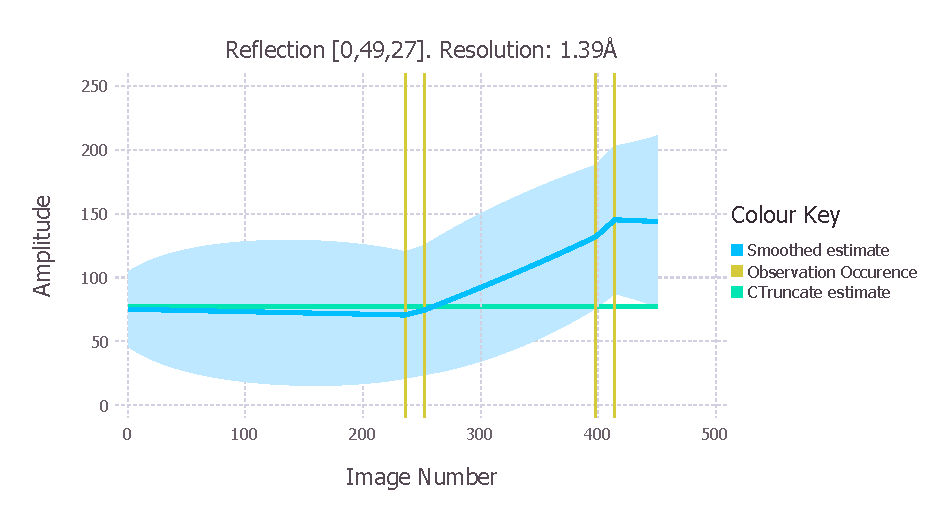
\includegraphics[width=\textwidth]{figures/datared/SmoothedPlot_0,49,27_res1.pdf}
        \caption{}
        \label{fig:Amplitude estimates ref 0,49,27 - insulin}
    \end{subfigure}
    \\
    \begin{subfigure}[b]{1.0\textwidth}
        \centering
        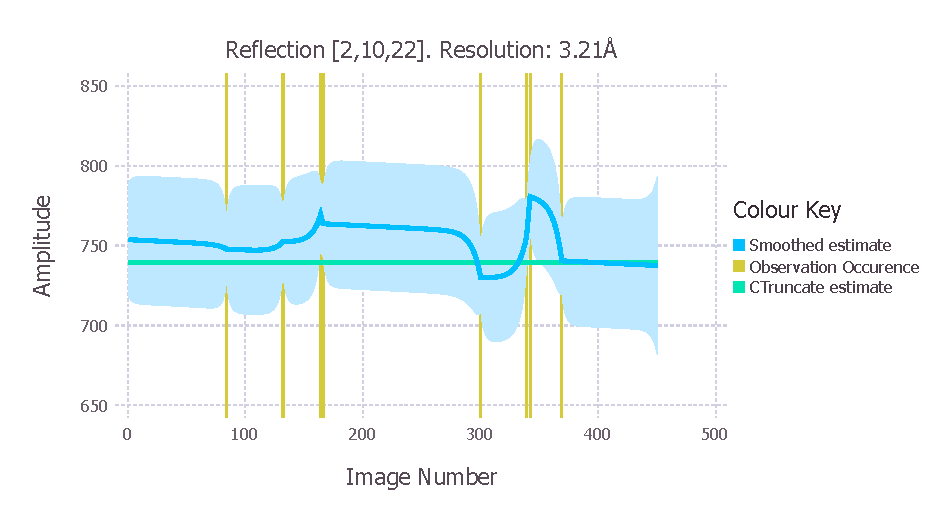
\includegraphics[width=\textwidth]{figures/datared/SmoothedPlot_2,10,22_res3.pdf}
        \caption{}
        \label{fig:Amplitude estimates ref 2,10,22 - insulin}
    \end{subfigure}
    \caption{Amplitude estimates for four different reflections observed in the insulin dataset using the forward-backward algorithm (blue solid line).
    The estimate produced with CTRUNCATE is shown in turquoise.
    The estimates all agree within the 95\% confidence interval (light blue shaded region) determined by the forward-backward algorithm.
    (a), (b) and (c) exhibit somewhat smooth changes in the amplitude behaviour, whereas (d) shows very sharp and irregular changes, which are likely to be unphysical.}
    \label{fig:Amplitude estimates - insulin}
\end{figure}

\subsubsection{Refinement results}
\label{subs:Refinement results - insulin}
The initial amplitude estimates resulting from the forward-backward algorithm (FBA) were processed with 10 cycles of rigid body refinement with REFMAC \cite{murshudov2011refmac5} using a deposited insulin structure (PDB code 2BN3) as the input model.
This was followed by 10 cycles of restrained refinement.
The same refinement process was performed with data processed with AIMLESS \cite{evans2013} and CTRUNCATE (ACT pipeline)\cite{winn2011} (i.e. no processing with the forward-backward algorithm).
The resulting electron density maps contoured at the 3$\sigma$ for selected residues are shown in Figure~\ref{fig:Electron density maps - insulin}.
The maps are practically identical for the two different data reduction pipelines, which is the case for the rest of the structure.
\begin{figure}
	\centering
    \begin{subfigure}[b]{1.0\textwidth}
        \centering
        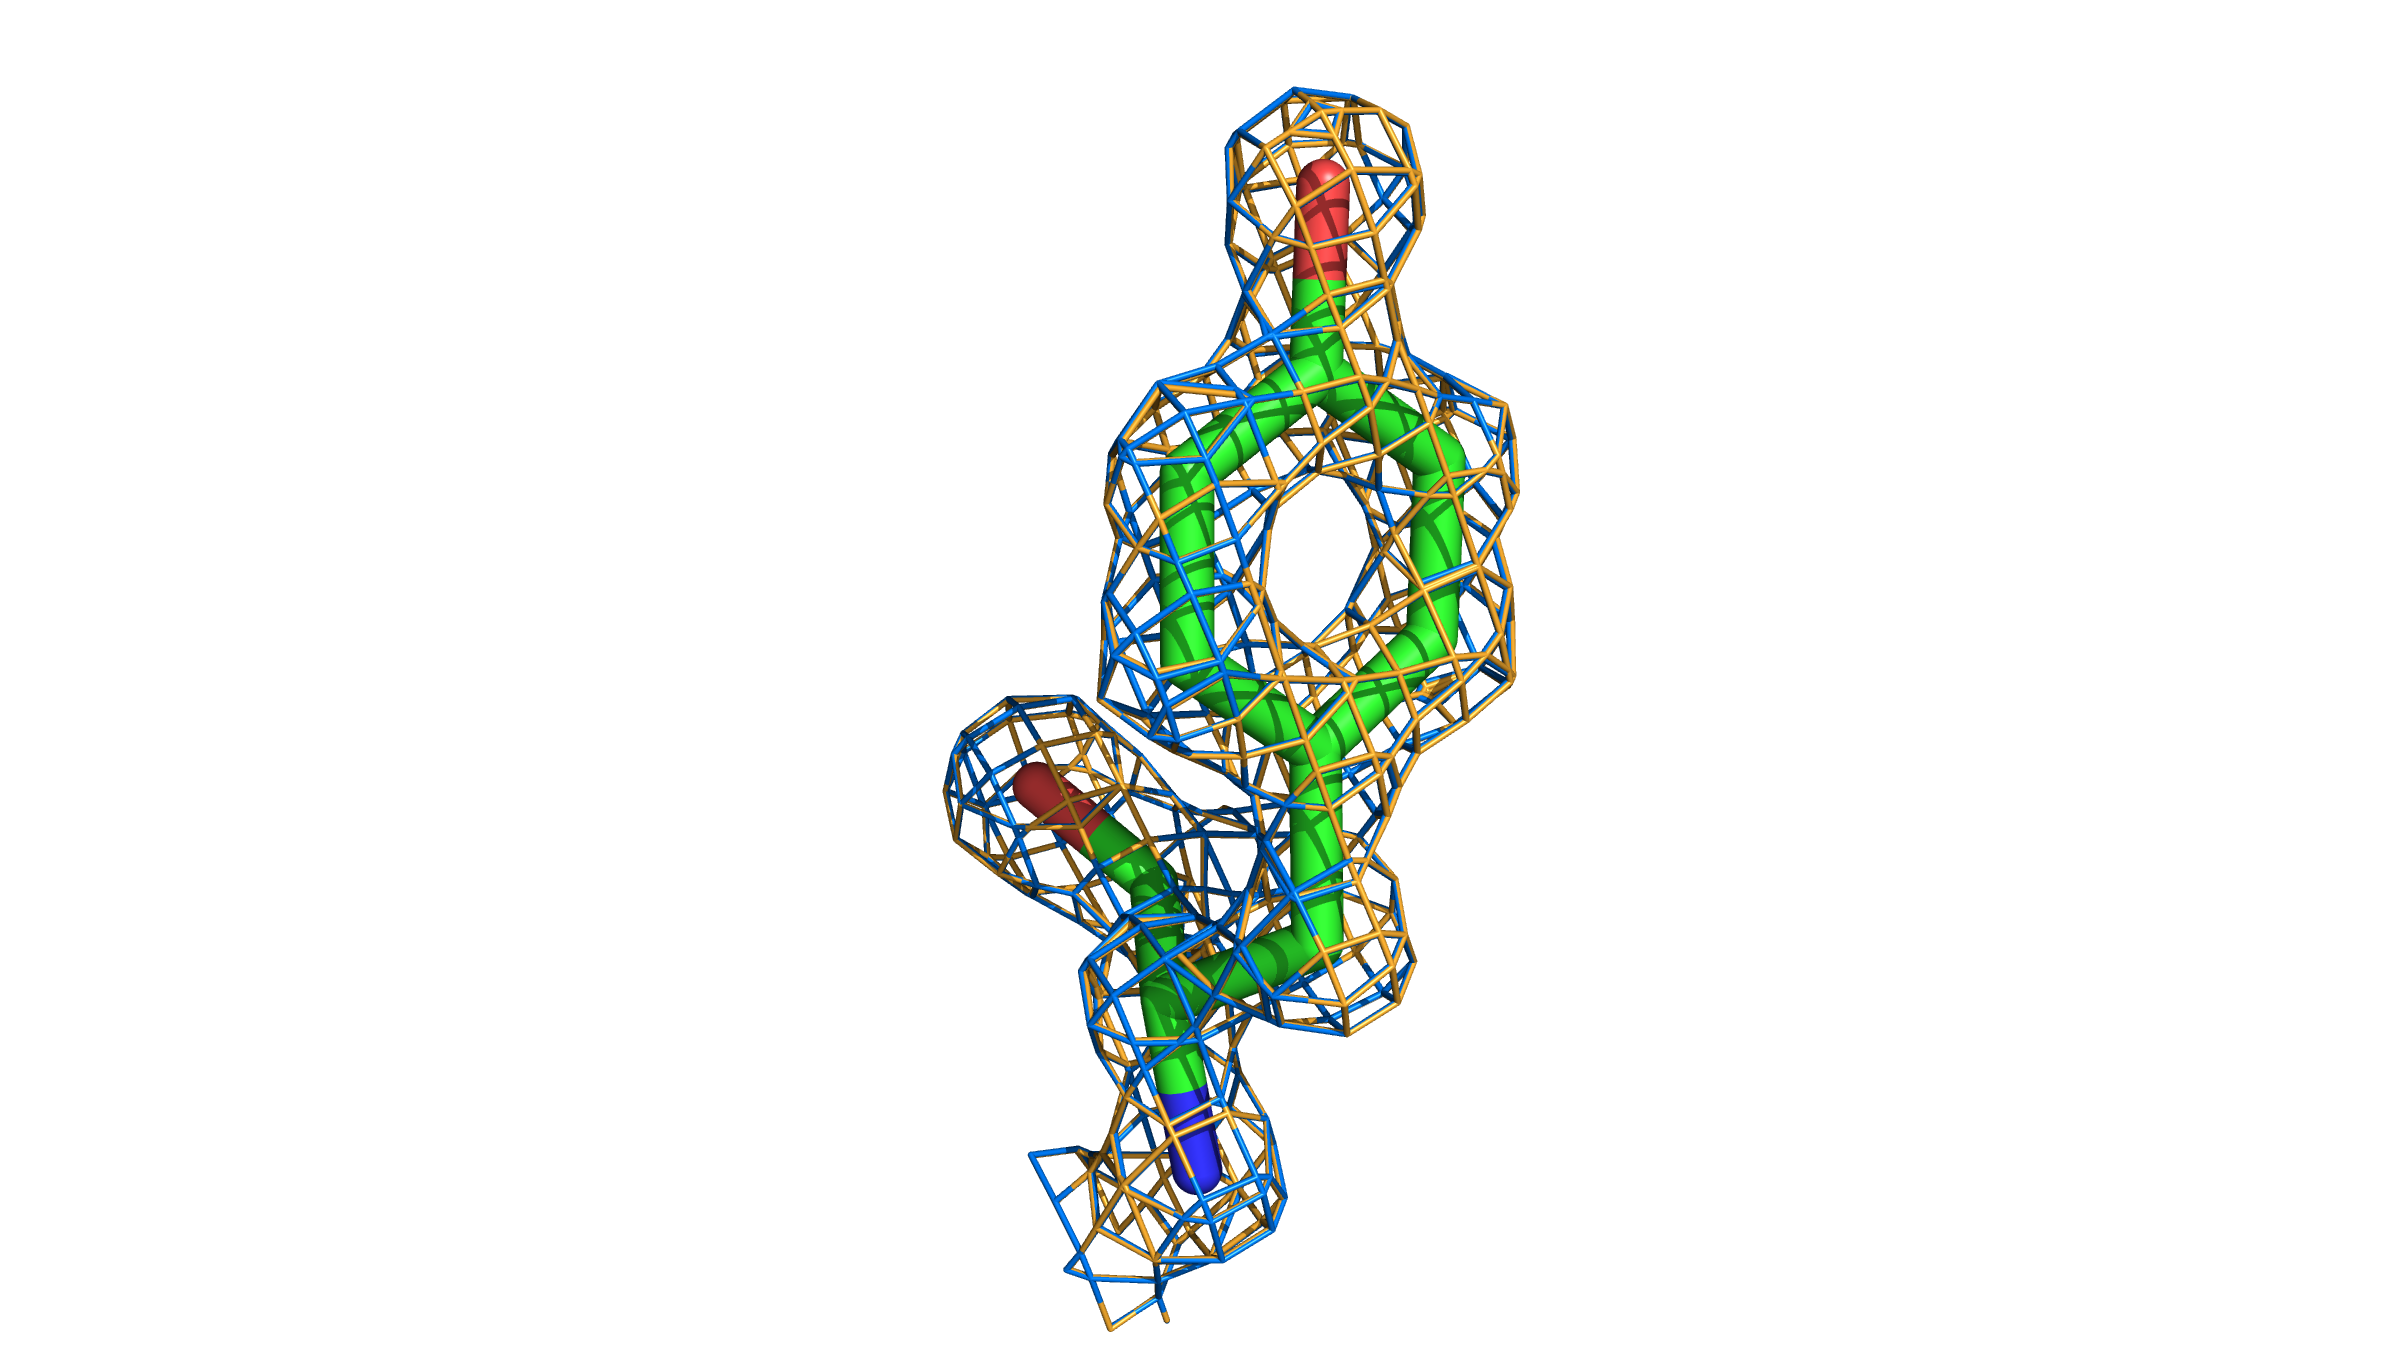
\includegraphics[width=\textwidth]{figures/datared/tyrosine_insulin.png}
        \caption{}
        \label{fig:Tyrosine residue - insulin}
    \end{subfigure}
    \\
	\begin{subfigure}[b]{1.0\textwidth}
        \centering
        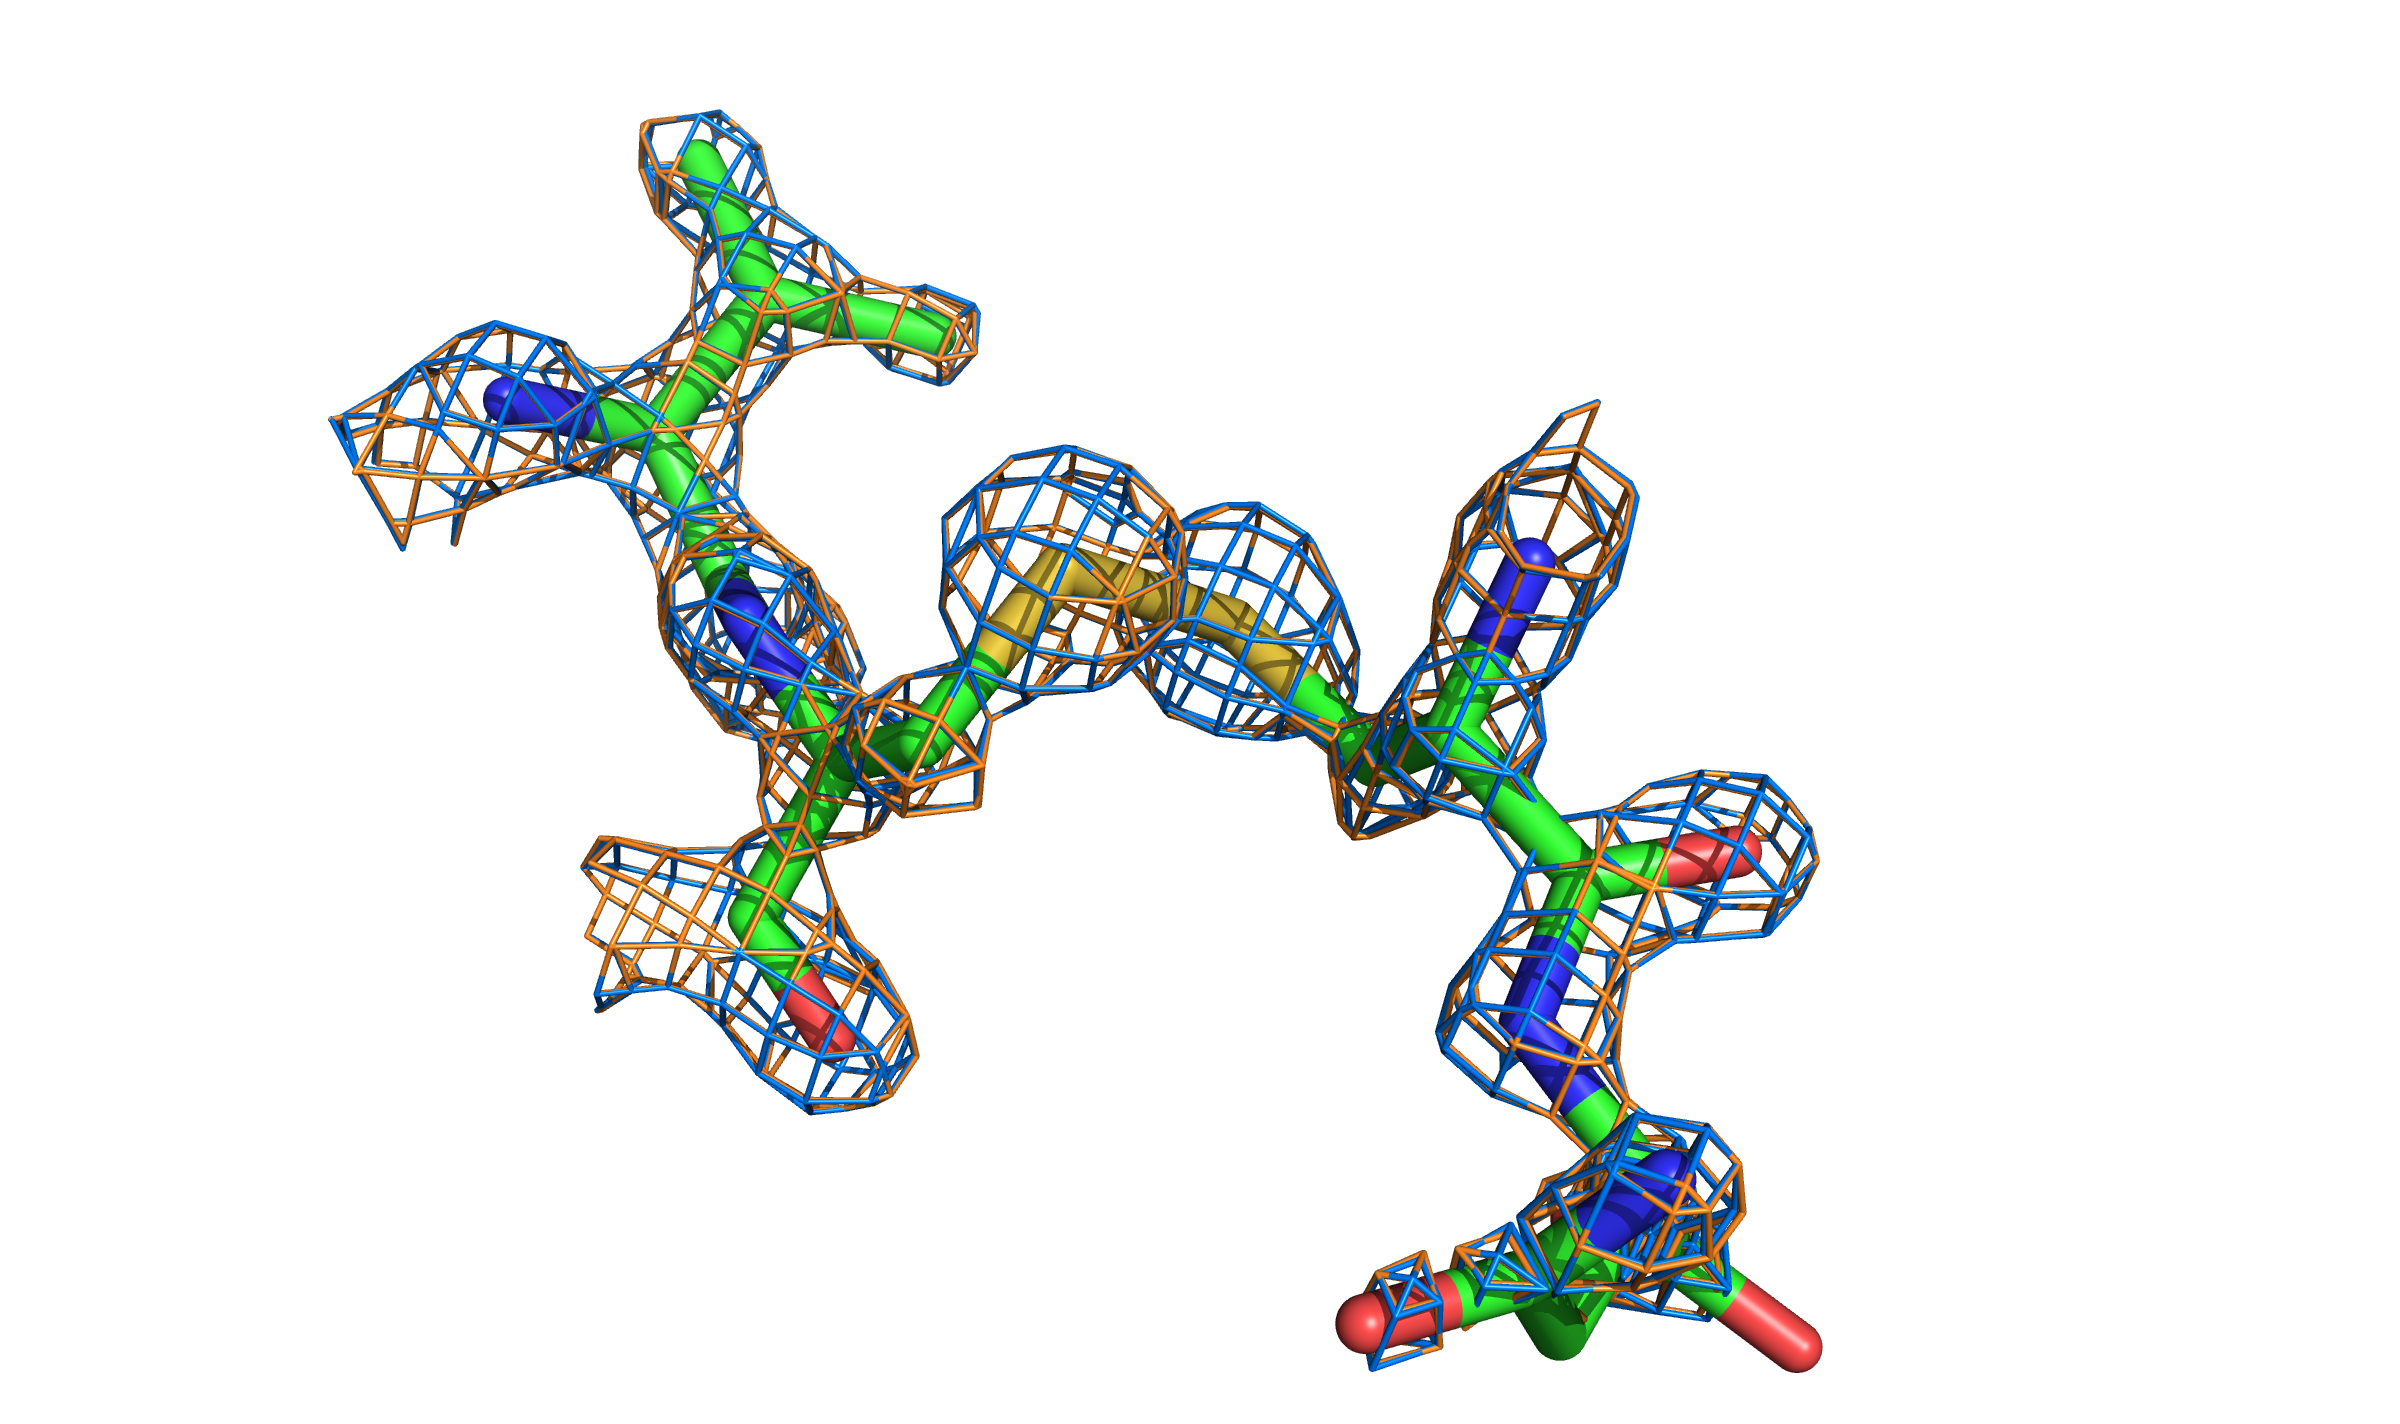
\includegraphics[width=\textwidth]{figures/datared/disulphide_insulin.png}
        \caption{}
        \label{fig:Disulpide bond - insulin}
    \end{subfigure}
    \caption{2F$_{\text{o}}$ - F$_{\text{c}}$ electron density maps contoured at the 3$\sigma$ level for the ACT pipeline (blue) and the FBA pipeline (orange) with the insulin structure obtained after refinement with REFMAC with data processed via the ACT pipeline.
    (a) Tyrosine residue.
    (b) Disulphide bond.
    The electron density maps are practically identical and this is representative of the density around the entire structure.}
    \label{fig:Electron density maps - insulin}
\end{figure}

A difference map was also calculated to determine where the major differences were using the two different data reduction pipelines.
The differences were calculated between the resulting amplitudes from the ACT and FBA pipelines, rather than the calculated amplitudes after refinement.
Phases were obtained from the model obtained after refinement with the data processed using the ACT pipeline.
Figure~\ref{fig:Difference electron density map - insulin} displays the resulting difference map contoured at the 3$\sigma$ level along with the full insulin structure from which the phases were obtained.
The difference electron density is distributed quite uniformly over the unit cell rather than large differences overlapping the structure.
This supports the result shown above that the two methods give practically identical electron density for the structure.
\begin{figure}
    \begin{subfigure}[b]{1.0\textwidth}
        \centering
        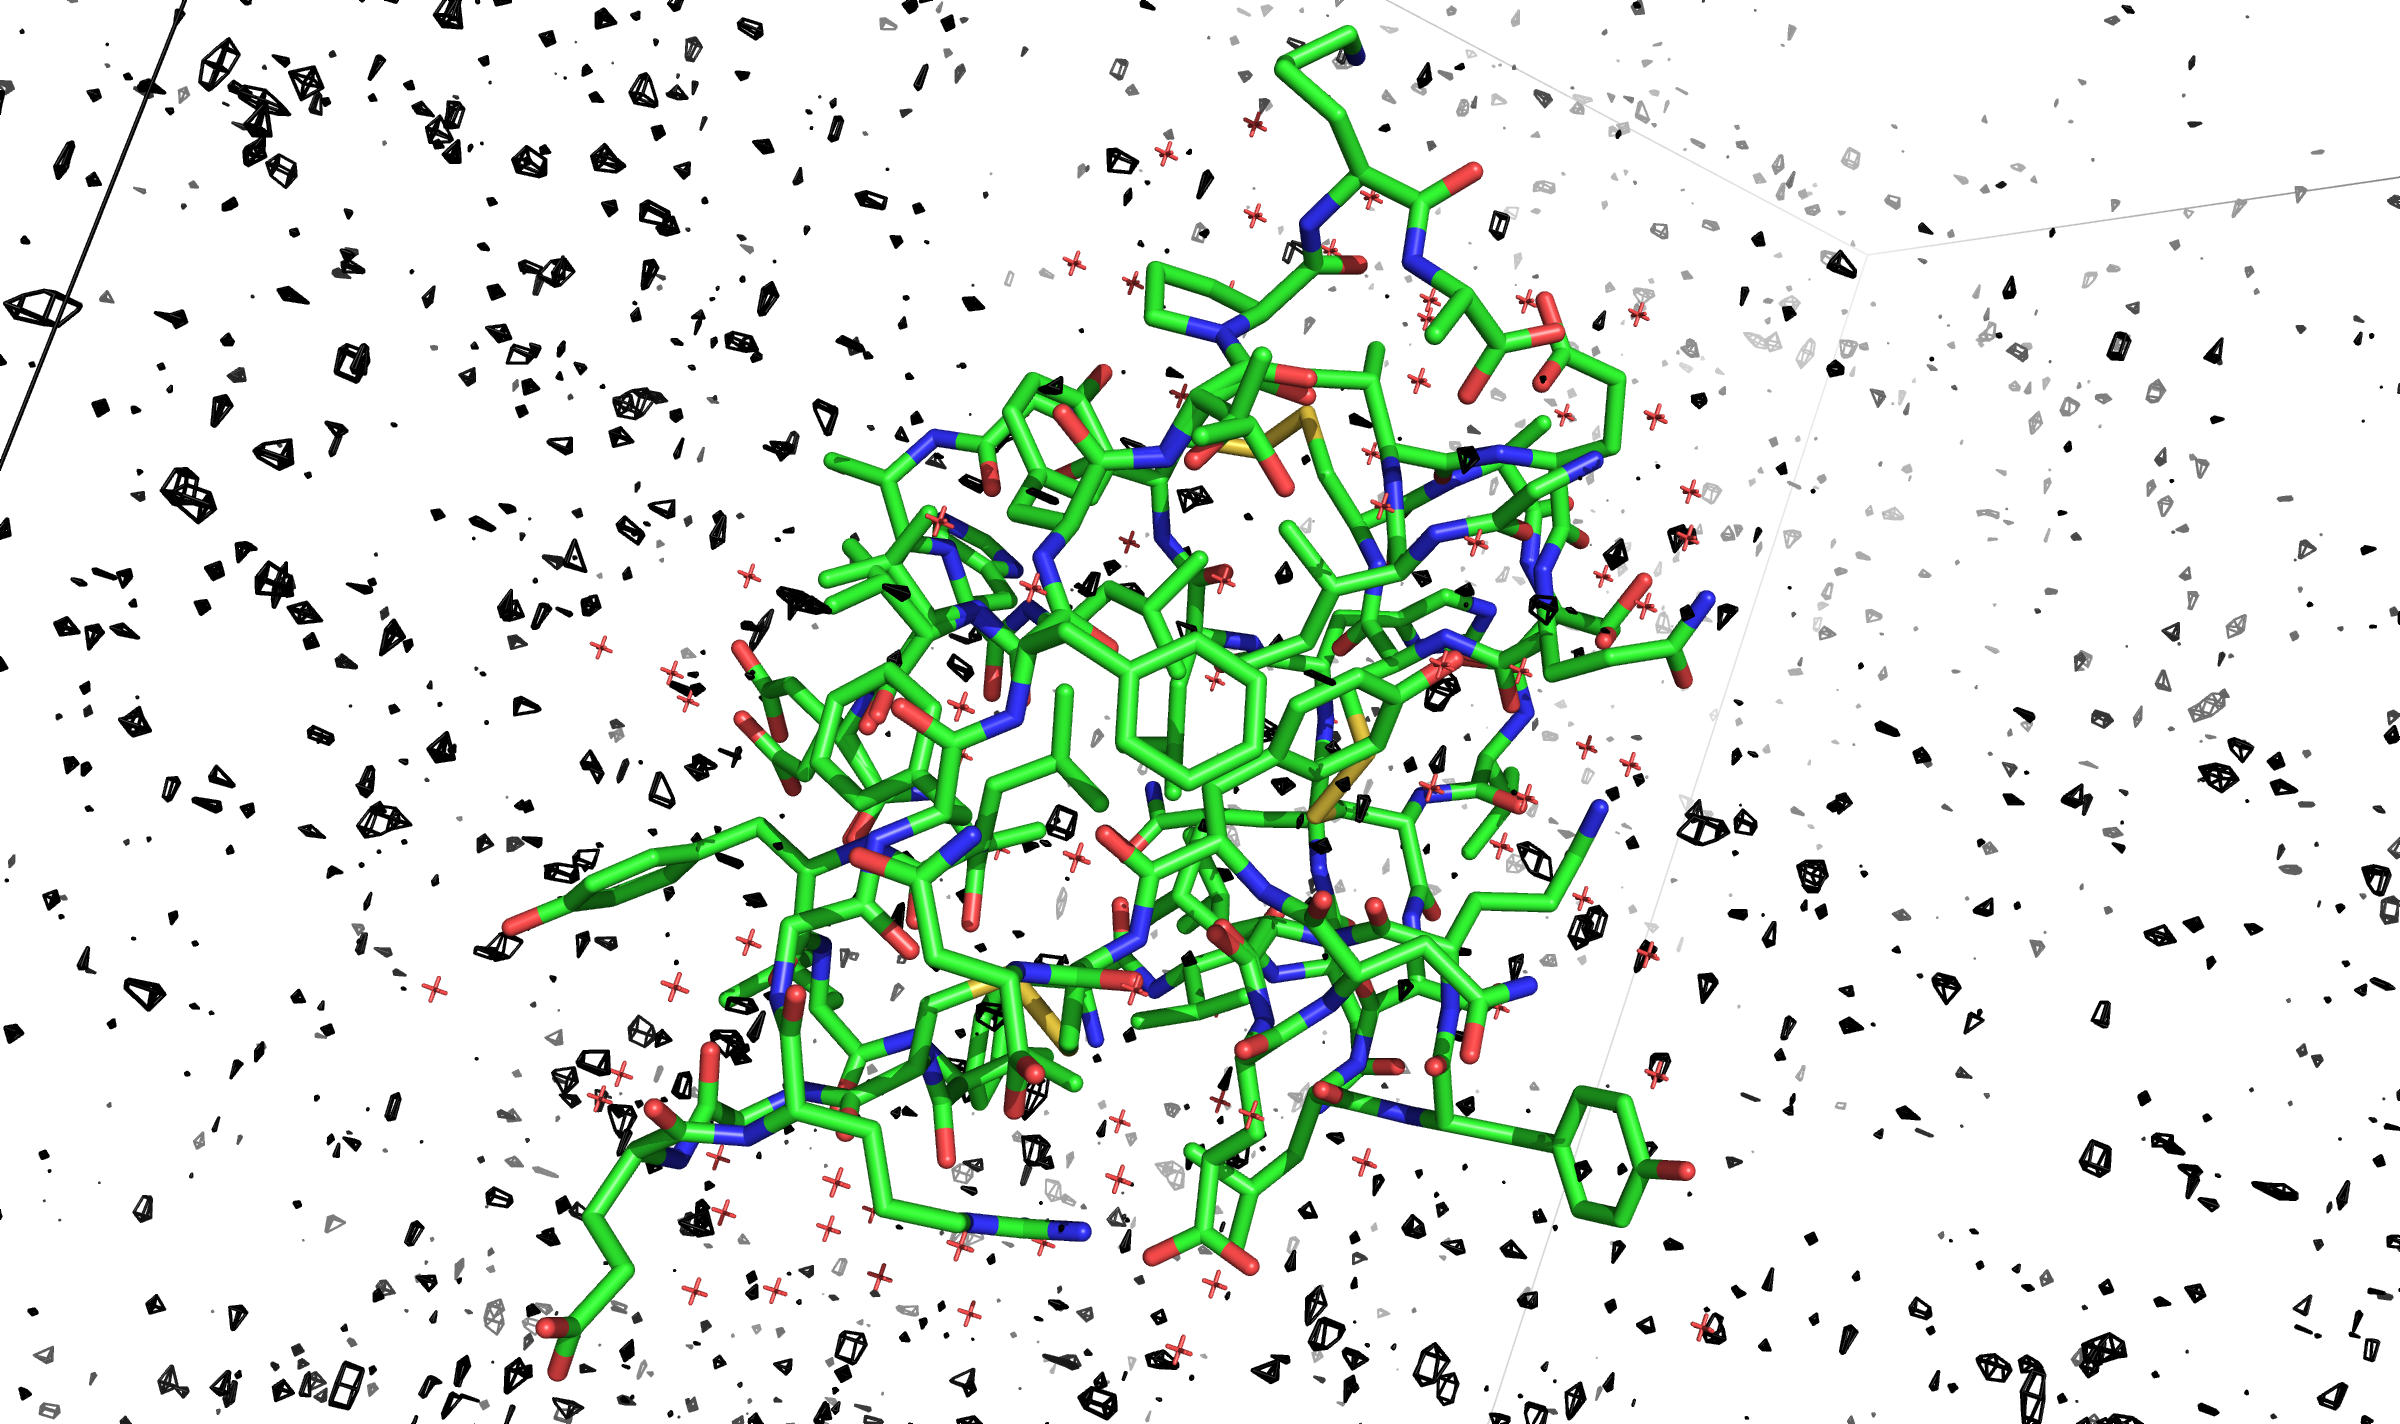
\includegraphics[width=\textwidth]{figures/datared/diff_aim_fba_insulin_seq_cnvc.png}
    \end{subfigure}
    \caption{Difference electron density map (black mesh) contoured at the 3$\sigma$ level between the amplitudes resulting from the ACT pipeline and the FBA pipeline using the phases obtained from the model resulting from refinement with the data processed using the ACT pipeline.
    The insulin structure from which the phases were obtained is also present.
    The difference density is uniformly distributed throughout the unit cell and no large differences can be seen overlapping the structure.
    This suggests that the two methods would result in the same structure as evidence by the electron density maps in Figure~\ref{fig:Electron density maps - insulin}.}
    \label{fig:Difference electron density map - insulin}
\end{figure}

Refinement statistics for both pipelines are shown in Table \ref{tab:Refinement statistics - insulin}.
Overall the statistics are quite similar but they are consistently better for the ACT pipeline.
It is likely that the FBA results can be improved by merging the amplitude estimates for symmetry related reflections after the algorithm has been applied to each observation individually, as described in section \ref{subs:Forward-backward algorithm - insulin}.
Another difference between the two pipelines is that the FBA pipeline does not include any outlier rejection whereas AIMLESS does.
This is likely to be reason why there were more reflections at the end of data reduction using the FBA pipeline (16261) compared to that using the ACT pipeline (16233).

\begin{table}[ht!]
	\caption{Final refinement statistics for data processed with the ACT and FBA pipelines}
	\centering
	\begin{tabular}{p{4cm} | p{2.5cm} | p{2.5cm}}
		   & ACT & FBA  \\
		\hline
		R work                      & 0.165   & 0.171 \\
		R free                      & 0.177   & 0.182 \\
		RMS bond length (\AA)       & 0.029   & 0.030 \\
        RMS Bond Angle ($^{\circ}$) & 2.493   & 2.552 \\
		\hline
	\end{tabular}
	\label{tab:Refinement statistics - insulin}
\end{table}

\subsection{Protein-DNA complex - C.Esp1396I}
\label{sub:Protein-DNA complex - C.Esp1396I}

\subsubsection{Scale and B factors}
\label{subs:Scale and B factors - C.Esp1396I}
Data were collected from a crystal of the bacterial protein-DNA complex (C.Esp1396I) as described in \cite{bury2015radiation} (Figure~\ref{fig:C.Esp1396I structure} ).
\begin{figure}[ht!]
    \centering
    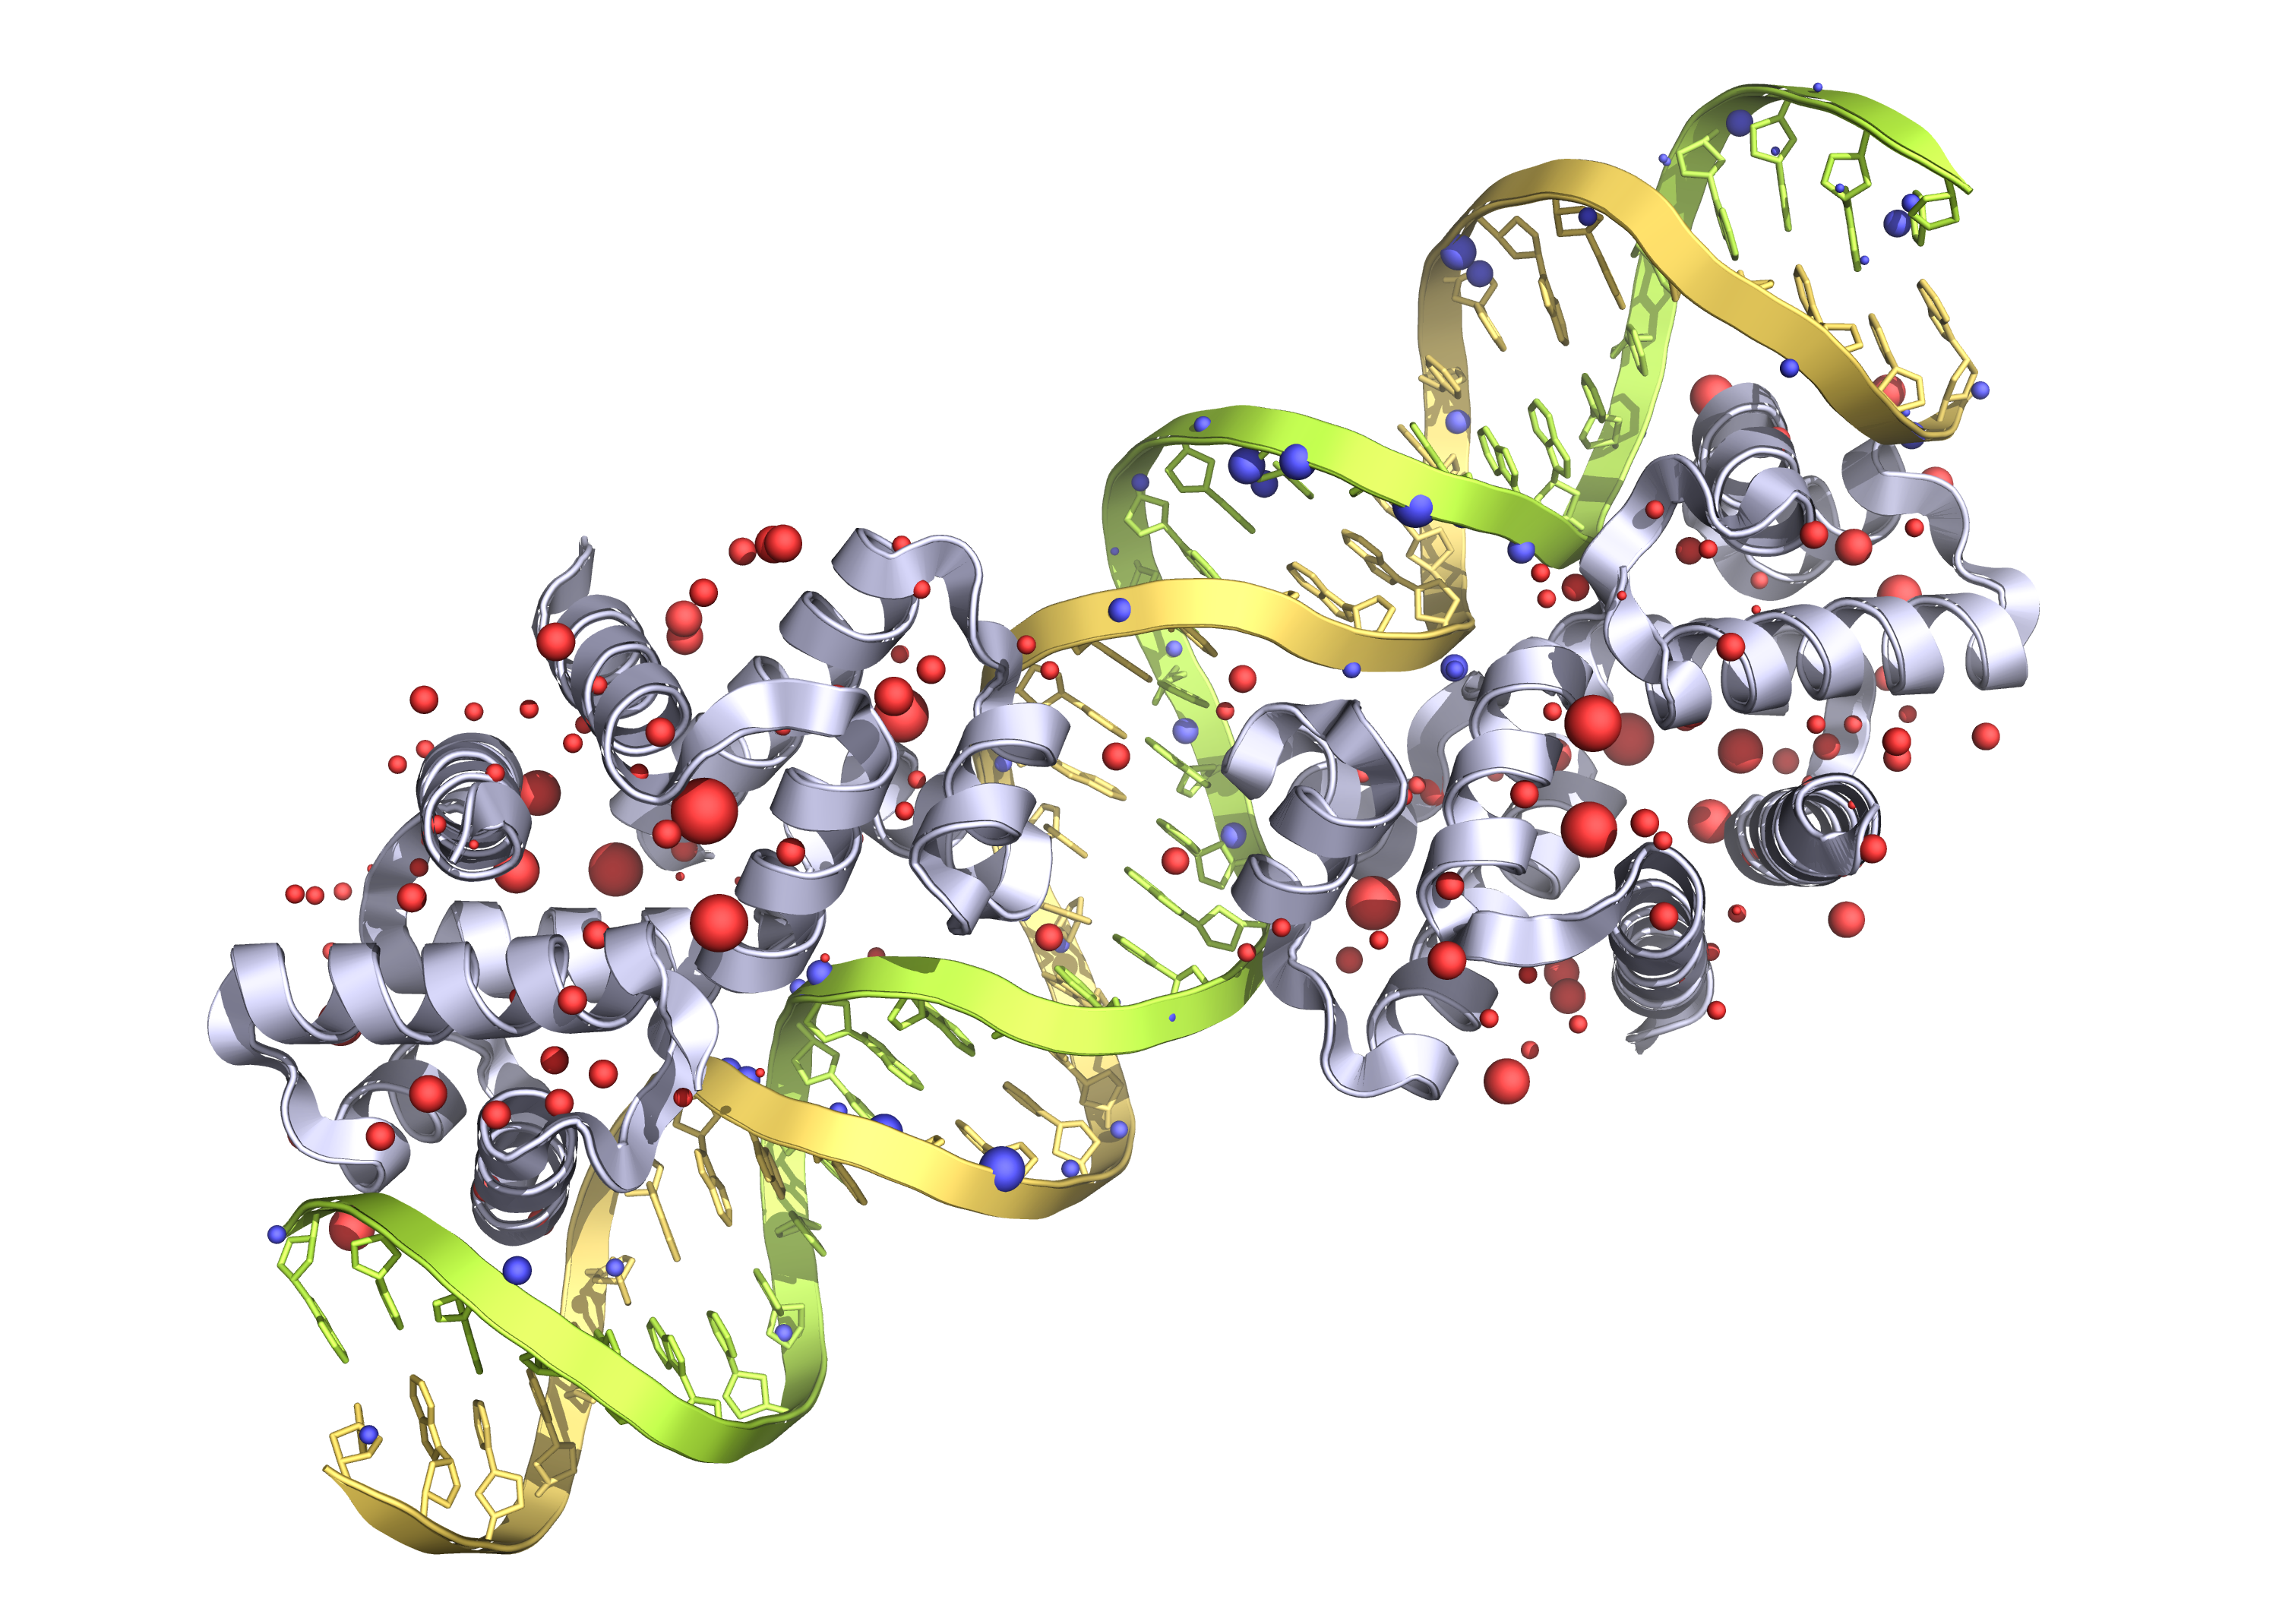
\includegraphics[width=1.0\textwidth]{figures/datared/JSRcoverpic_nobackground.png}
    \caption{Structure of the C.Esp1396I protein-DNA complex.
    The spheres show sites of specific radiation damage at a dose of 44.6$\,$MGy.
    The radii of the spheres are proportional to the electron density loss and the spheres closer/further than 2$\,$\AA from the DNA strands are coloured blue/red \cite{bury2015radiation}.}
    \label{fig:C.Esp1396I structure}
\end{figure}
The atomic composition used to provide expected intensity values was obtained from the PDB structure 4X4B.
The B factors were calculated as described above and are shown in Figure~\ref{fig:B factors per image - C.Esp1396I}.
Four outliers that were removed in the outlier rejection procedure are clearly visible in Figure~\ref{fig:B factors per image before outlier removal - C.Esp1396I} with B factor values of zero.
The initial B factor is much higher for the C.Esp1396I structure (57.69) than it is for the insulin structure (12.19).
In contrast to the behaviour observed with the insulin dataset, the B factor for the C.Esp1396I structure decreases linearly throughout the dataset (Figure~\ref{fig:B factors per image after outlier removal - C.Esp1396I}).
The assumption of a linear behaviour of the B-factor is again justified (Figure~\ref{fig:Gaussian B factor plots - C.Esp1396I} )
\begin{figure}
    \centering
    \begin{subfigure}[b]{1.0\textwidth}
            \centering
            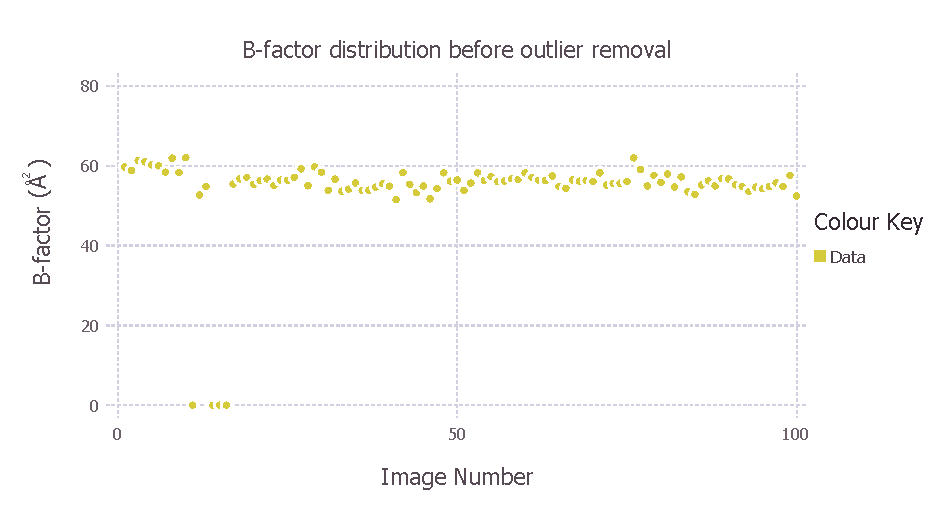
\includegraphics[width=\textwidth]{figures/datared/BFac_Plot_Before_outlier_removal_cprot.pdf}
            \caption{}
            \label{fig:B factors per image before outlier removal - C.Esp1396I}
    \end{subfigure}
    \\
    \begin{subfigure}[b]{1.0\textwidth}
            \centering
            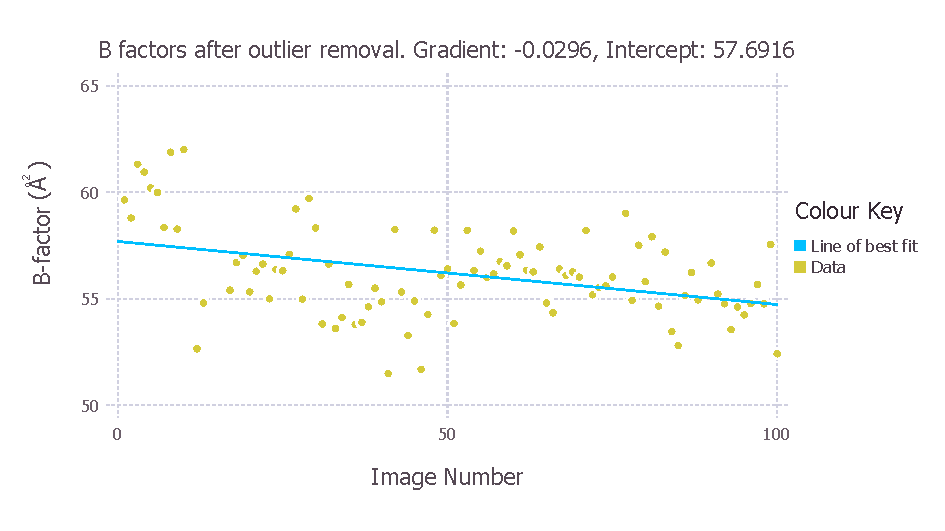
\includegraphics[width=\textwidth]{figures/datared/BFac_Plot_After_outlier_removal_cprot.pdf}
            \caption{}
            \label{fig:B factors per image after outlier removal - C.Esp1396I}
    \end{subfigure}
    \caption{Calculated B factors for each image in the C.Esp1396I dataset.
    (a) Distribution before outlier removal.
    (b) Distribution after outlier removal.
    The line of best fit (blue solid line) with gradient, $\Delta B$ = -0.0296 and intercept = 57.5916, is overlaid on the data.}
    \label{fig:B factors per image - C.Esp1396I}
\end{figure}

\begin{figure}
    \centering
    \begin{subfigure}[b]{1.0\textwidth}
            \centering
            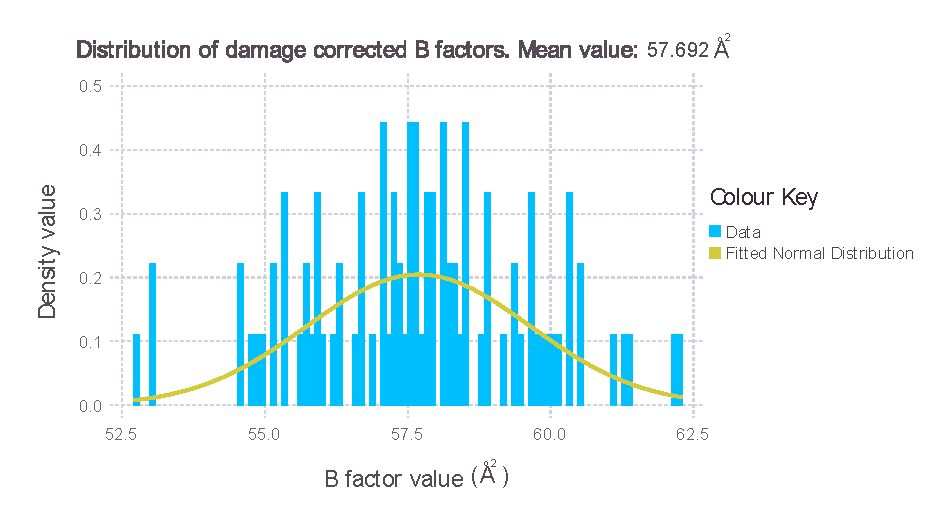
\includegraphics[width=\textwidth]{figures/datared/BFac_Distribution_cprot.pdf}
            \caption{}
            \label{fig:Damage corrected B factor distribution - C.Esp1396I}
    \end{subfigure}
    \\
    \begin{subfigure}[b]{1.0\textwidth}
            \centering
            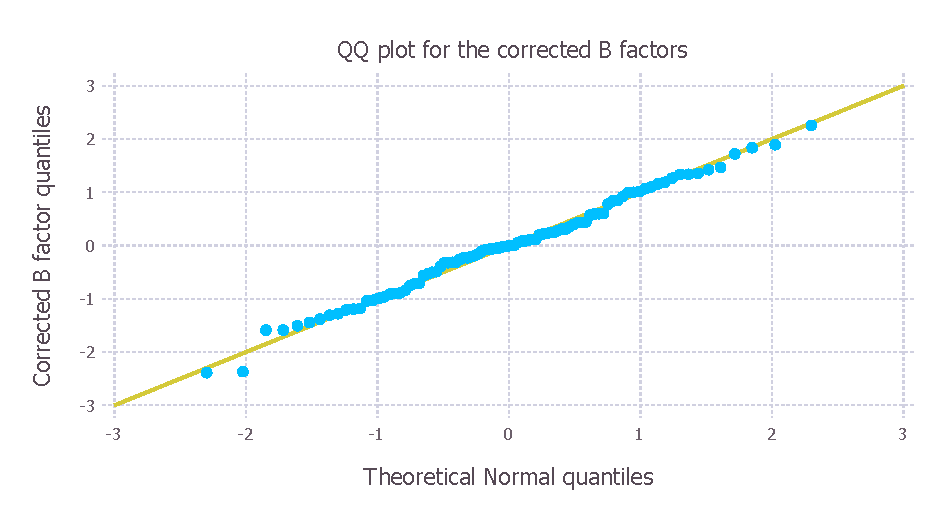
\includegraphics[width=\textwidth]{figures/datared/BFac_QQplot_cprot.pdf}
            \caption{Dose at which maximum curvature is reached}
            \label{fig:B factor QQ plot - C.Esp1396I}
    \end{subfigure}
    \caption{(a) Histogram of damage corrected B factors for the C.Esp1396I structure.
    (b) QQ plot for the damage corrected B factors.
    The linearity of the points in the QQ plot support the Gaussian approximation in the histogram, suggesting that the B factors change linearly.}
    \label{fig:Gaussian B factor plots - C.Esp1396I}
\end{figure}

The calculated scale factors are shown in Figure~\ref{fig:Scale factors per image - C.Esp1396I}.
As with the insulin dataset, no specific outlier rejection was carried out on the scale factors so the only scale factors that were rejected were the ones that corresponded to the same images on which the rejected B factors were found.
This corresponded to the four scale factors with a value of 1 in Figure~\ref{fig:Scale factors per image before outlier removal - C.Esp1396I}.
The resulting scale factors (Figure~\ref{fig:Scale factors per image after outlier removal - C.Esp1396I}) do not exhibit a constant behaviour as was the case with the insulin structure.
This means that the assumption of a constant scale factor is likely to give incorrect results.
The kernel density estimate in Figure~\ref{fig:Scale factor distribution after outlier removal - C.Esp1396I} shows that the scale factor distribution is bimodal and hence a single (constant) value does not represent the distribution very well.
A varying scale factor has not yet been implemented into the forward-backward algorithm and hence the mean value (0.0147) was used as the constant scale factor during processing.
\begin{figure}
    \centering
    \begin{subfigure}[b]{1.0\textwidth}
            \centering
            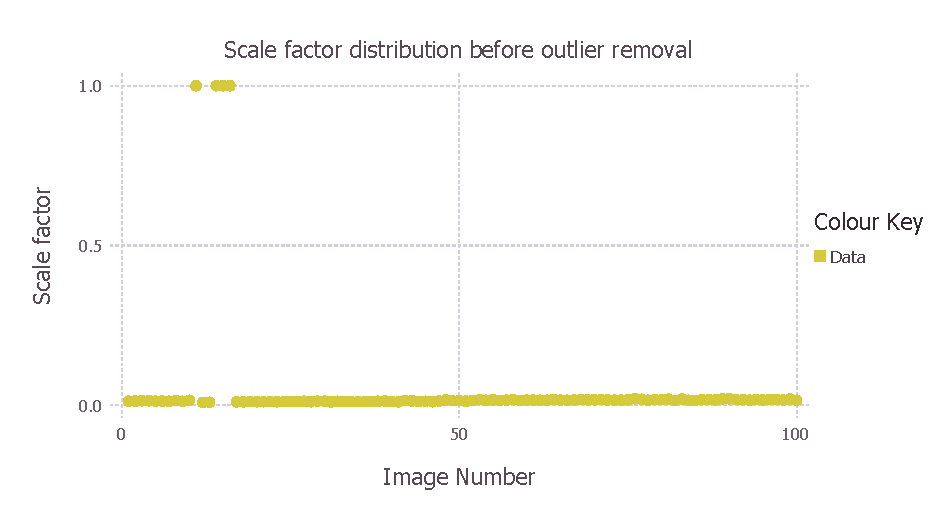
\includegraphics[width=\textwidth]{figures/datared/ScaleFac_Plot_Before_outlier_removal_cprot.pdf}
            \caption{}
            \label{fig:Scale factors per image before outlier removal - C.Esp1396I}
    \end{subfigure}
    \\
    \begin{subfigure}[b]{1.0\textwidth}
            \centering
            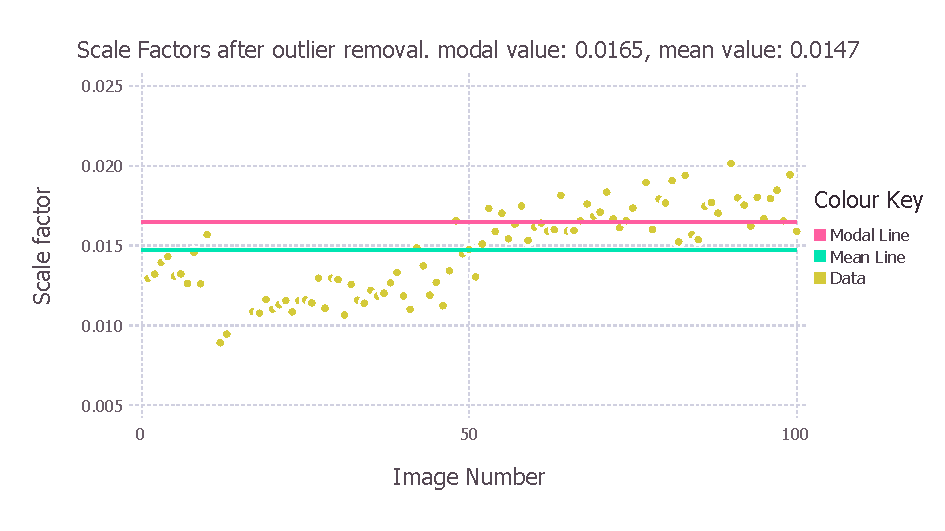
\includegraphics[width=\textwidth]{figures/datared/ScaleFac_Plot_After_outlier_removal_cprot.pdf}
            \caption{Dose at which maximum curvature is reached}
            \label{fig:Scale factors per image after outlier removal - C.Esp1396I}
    \end{subfigure}
    \caption{Calculated scale factors for each image in the C.Esp1396I dataset.
    (a) Distribution before outlier removal.
    (b) Distribution after outlier removal.
    The solid turquoise and solid pink lines represent the mean and mode of the distribution respectively.
    The scale factor is clearly not constant and shows an increasing trend throughout the experiment.
    This leads to differences in the mean and modal values of the distribution.}
    \label{fig:Scale factors per image - C.Esp1396I}
\end{figure}

\begin{figure}[ht!]
    \centering
    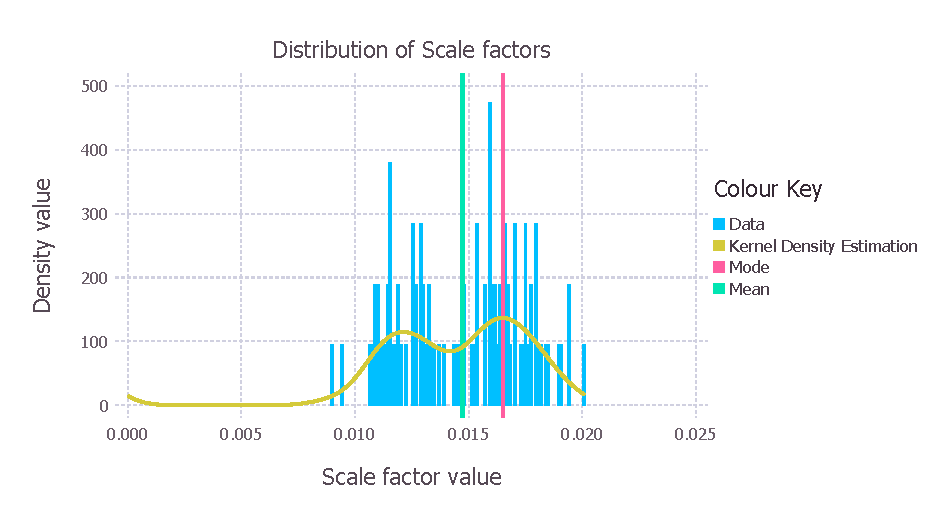
\includegraphics[width=1.0\textwidth]{figures/datared/ScaleFac_Distribution_cprot.pdf}
    \caption{Histogram of scale factors with the mean (solid turquoise line), mode (solid pink line) and kernel density estimation (solid gold line) overlaid.
    The bimodal distribution of the scale factor is clear from the kernel density estimate.}
    \label{fig:Scale factor distribution after outlier removal - C.Esp1396I}
\end{figure}

\subsubsection{Forward-backward algorithm}
\label{subs:Forward-backward algorithm - C.Esp1396I}
The forward-backward algorithm was carried out with the same parameters as defined for the insulin structure.
The only difference was that the Gaussian approximation was used as the process function for every reflection.
Furthermore the Bayesian inference method described in section \ref{sub:Weak Data} was not performed.
This was the algorithm came across numerical issues calculating the Rician approximation.
this is likely due to calculating the modified Bessel function of the first kind of order zero for arguments with high values.
Mathematically this function increases in an exponential manner, especially for large argument values.
This reaches a point where an error is thrown.
The Gaussian approximation does not rely on evaluating this function which is why it was used instead for all reflections.
Addressing this issue will require the program to check the size of the argument before evaluating it.

The amplitude estimates of two of the reflections resulting from the processing are shown in Figure~\ref{fig:Amplitude estimates - C.Esp1396I}.
As was the case with the insulin dataset, some reflections exhibit smooth behaviour (Figure~\ref{fig:Amplitude estimates ref 0,17,48 - C.Esp1396I}), whereas others show sharp changes that are likely to be due to imperfect scale factors (Figure~\ref{fig:Amplitude estimates ref 8,9,4 - C.Esp1396I}).
Due to the incorrect scale factor used for the images in the dataset, the CTRUNCATE and the FBA amplitude values do not agree.
\begin{figure}
    \centering
    \begin{subfigure}[b]{1.0\textwidth}
            \centering
            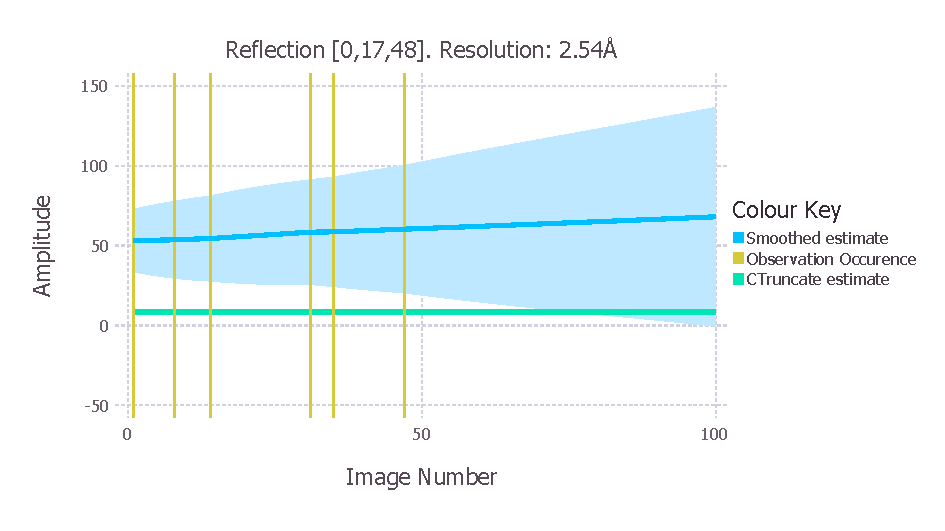
\includegraphics[width=\textwidth]{figures/datared/SmoothedPlot_0,17,48_res3.pdf}
            \caption{}
            \label{fig:Amplitude estimates ref 0,17,48 - C.Esp1396I}
    \end{subfigure}
    \\
    \begin{subfigure}[b]{1.0\textwidth}
            \centering
            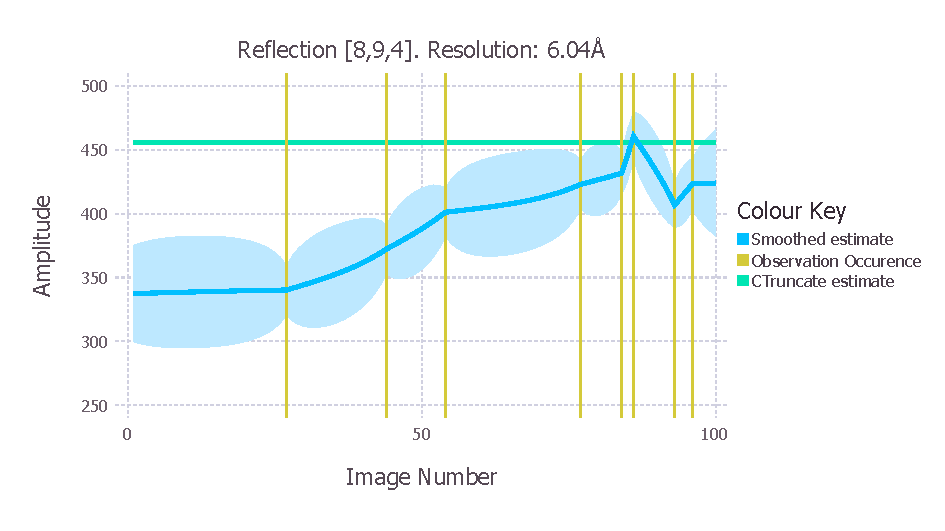
\includegraphics[width=\textwidth]{figures/datared/SmoothedPlot_8,9,4_res6.pdf}
            \caption{Dose at which maximum curvature is reached}
            \label{fig:Amplitude estimates ref 8,9,4 - C.Esp1396I}
    \end{subfigure}
    \caption{Amplitude estimates for two different reflections observed in the C.Esp1396I dataset using the forward-backward algorithm (blue solid line).
    The estimate produced with CTRUNCATE is shown in turquoise.
    The estimates using the two different pipelines do not agree and this is likely due to the incorrect scale factor used for the forward-backward algorithm.
    Reflection 8,9,4 in (b) also exhibits sharp changes in the amplitude, which are likely to be noise.}
    \label{fig:Amplitude estimates - C.Esp1396I}
\end{figure}

\subsubsection{Refinement results}
\label{subs:Refinement results - C.Esp1396I}
The initial amplitude estimates resulting from FBA and ACT were processed with 20 cycles of rigid body refinement with REFMAC \cite{murshudov2011refmac5} using a deposited insulin structure (PDB code 3CLC) as the input model.
This was followed by 20 cycles of restrained refinement.
The resulting electron density maps contoured at the 3$\sigma$ for selected residues are shown in Figure~\ref{fig:Electron density maps - C.Esp1396I} (the structural model is not shown because it requires more refinement to achieve suitable agreement with the data).
Once again the maps generally agree structurally but the overlap is less pronounced in this structure as it was for insulin.
This is expected because the amplitude values did not agree largely due to an incorrect scale factor used for the FBA.
\begin{figure}
    \centering
    \begin{subfigure}[b]{1.0\textwidth}
            \centering
            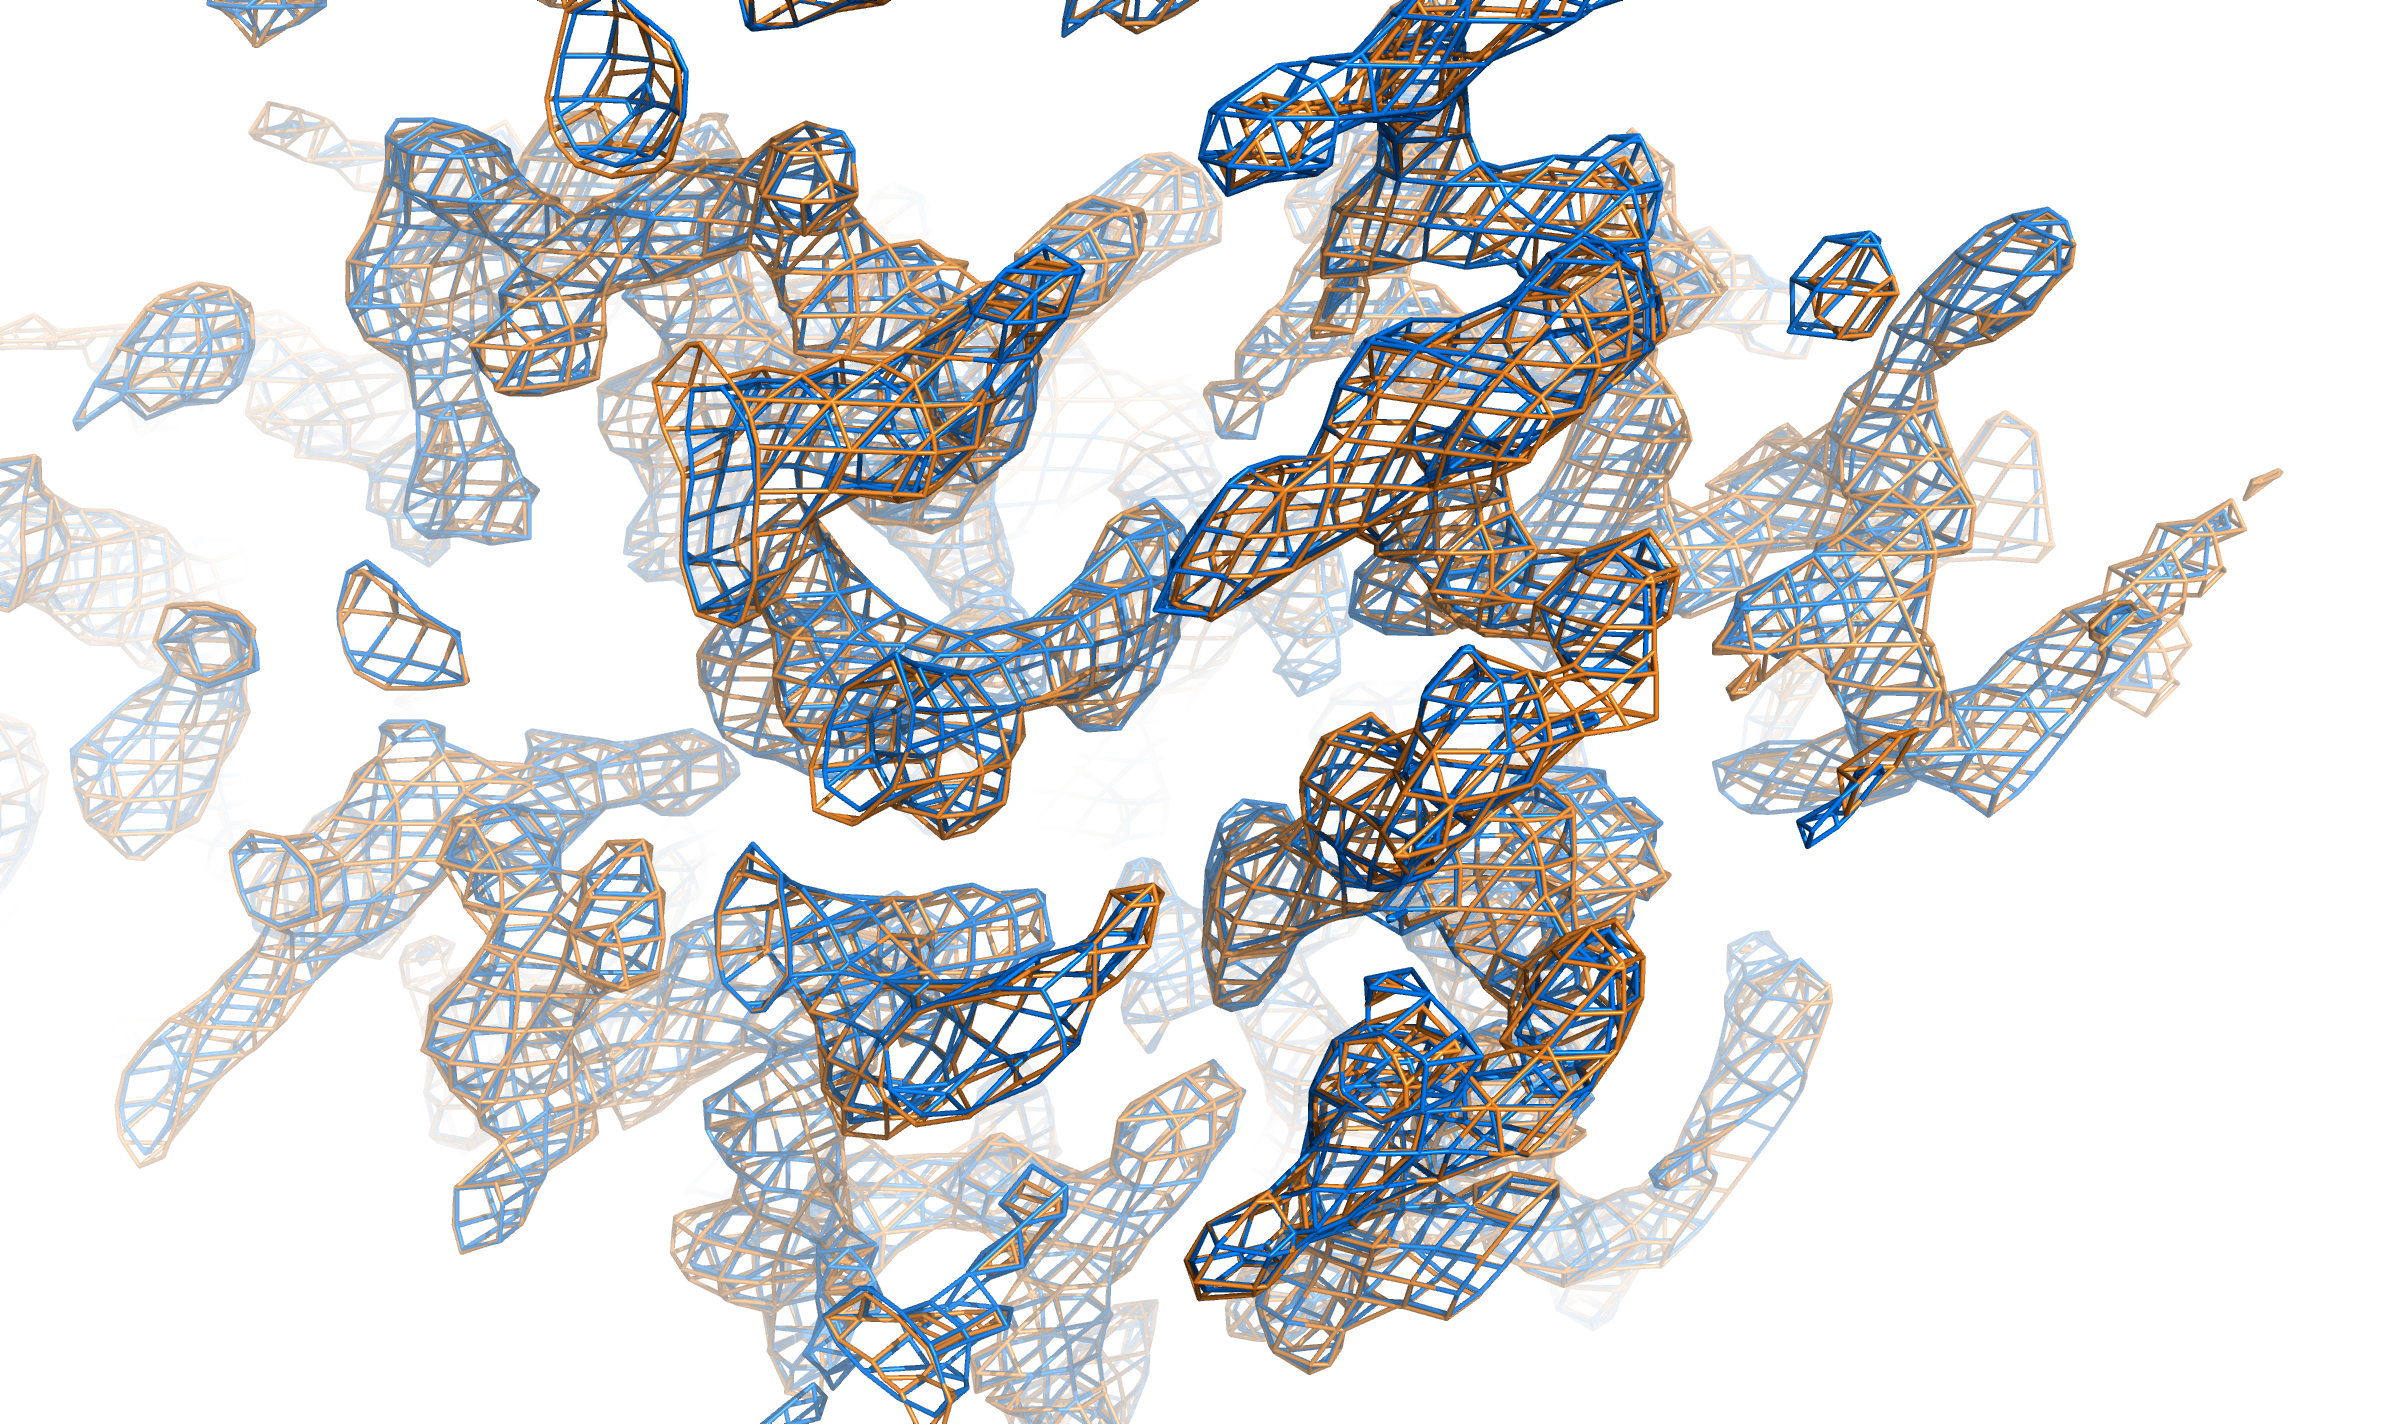
\includegraphics[width=\textwidth]{figures/datared/CPROT_elec_dens_comp1.png}
            \caption{}
            \label{fig:Electron density map 1 - C.Esp1396I}
    \end{subfigure}
    \\
    \begin{subfigure}[b]{1.0\textwidth}
            \centering
            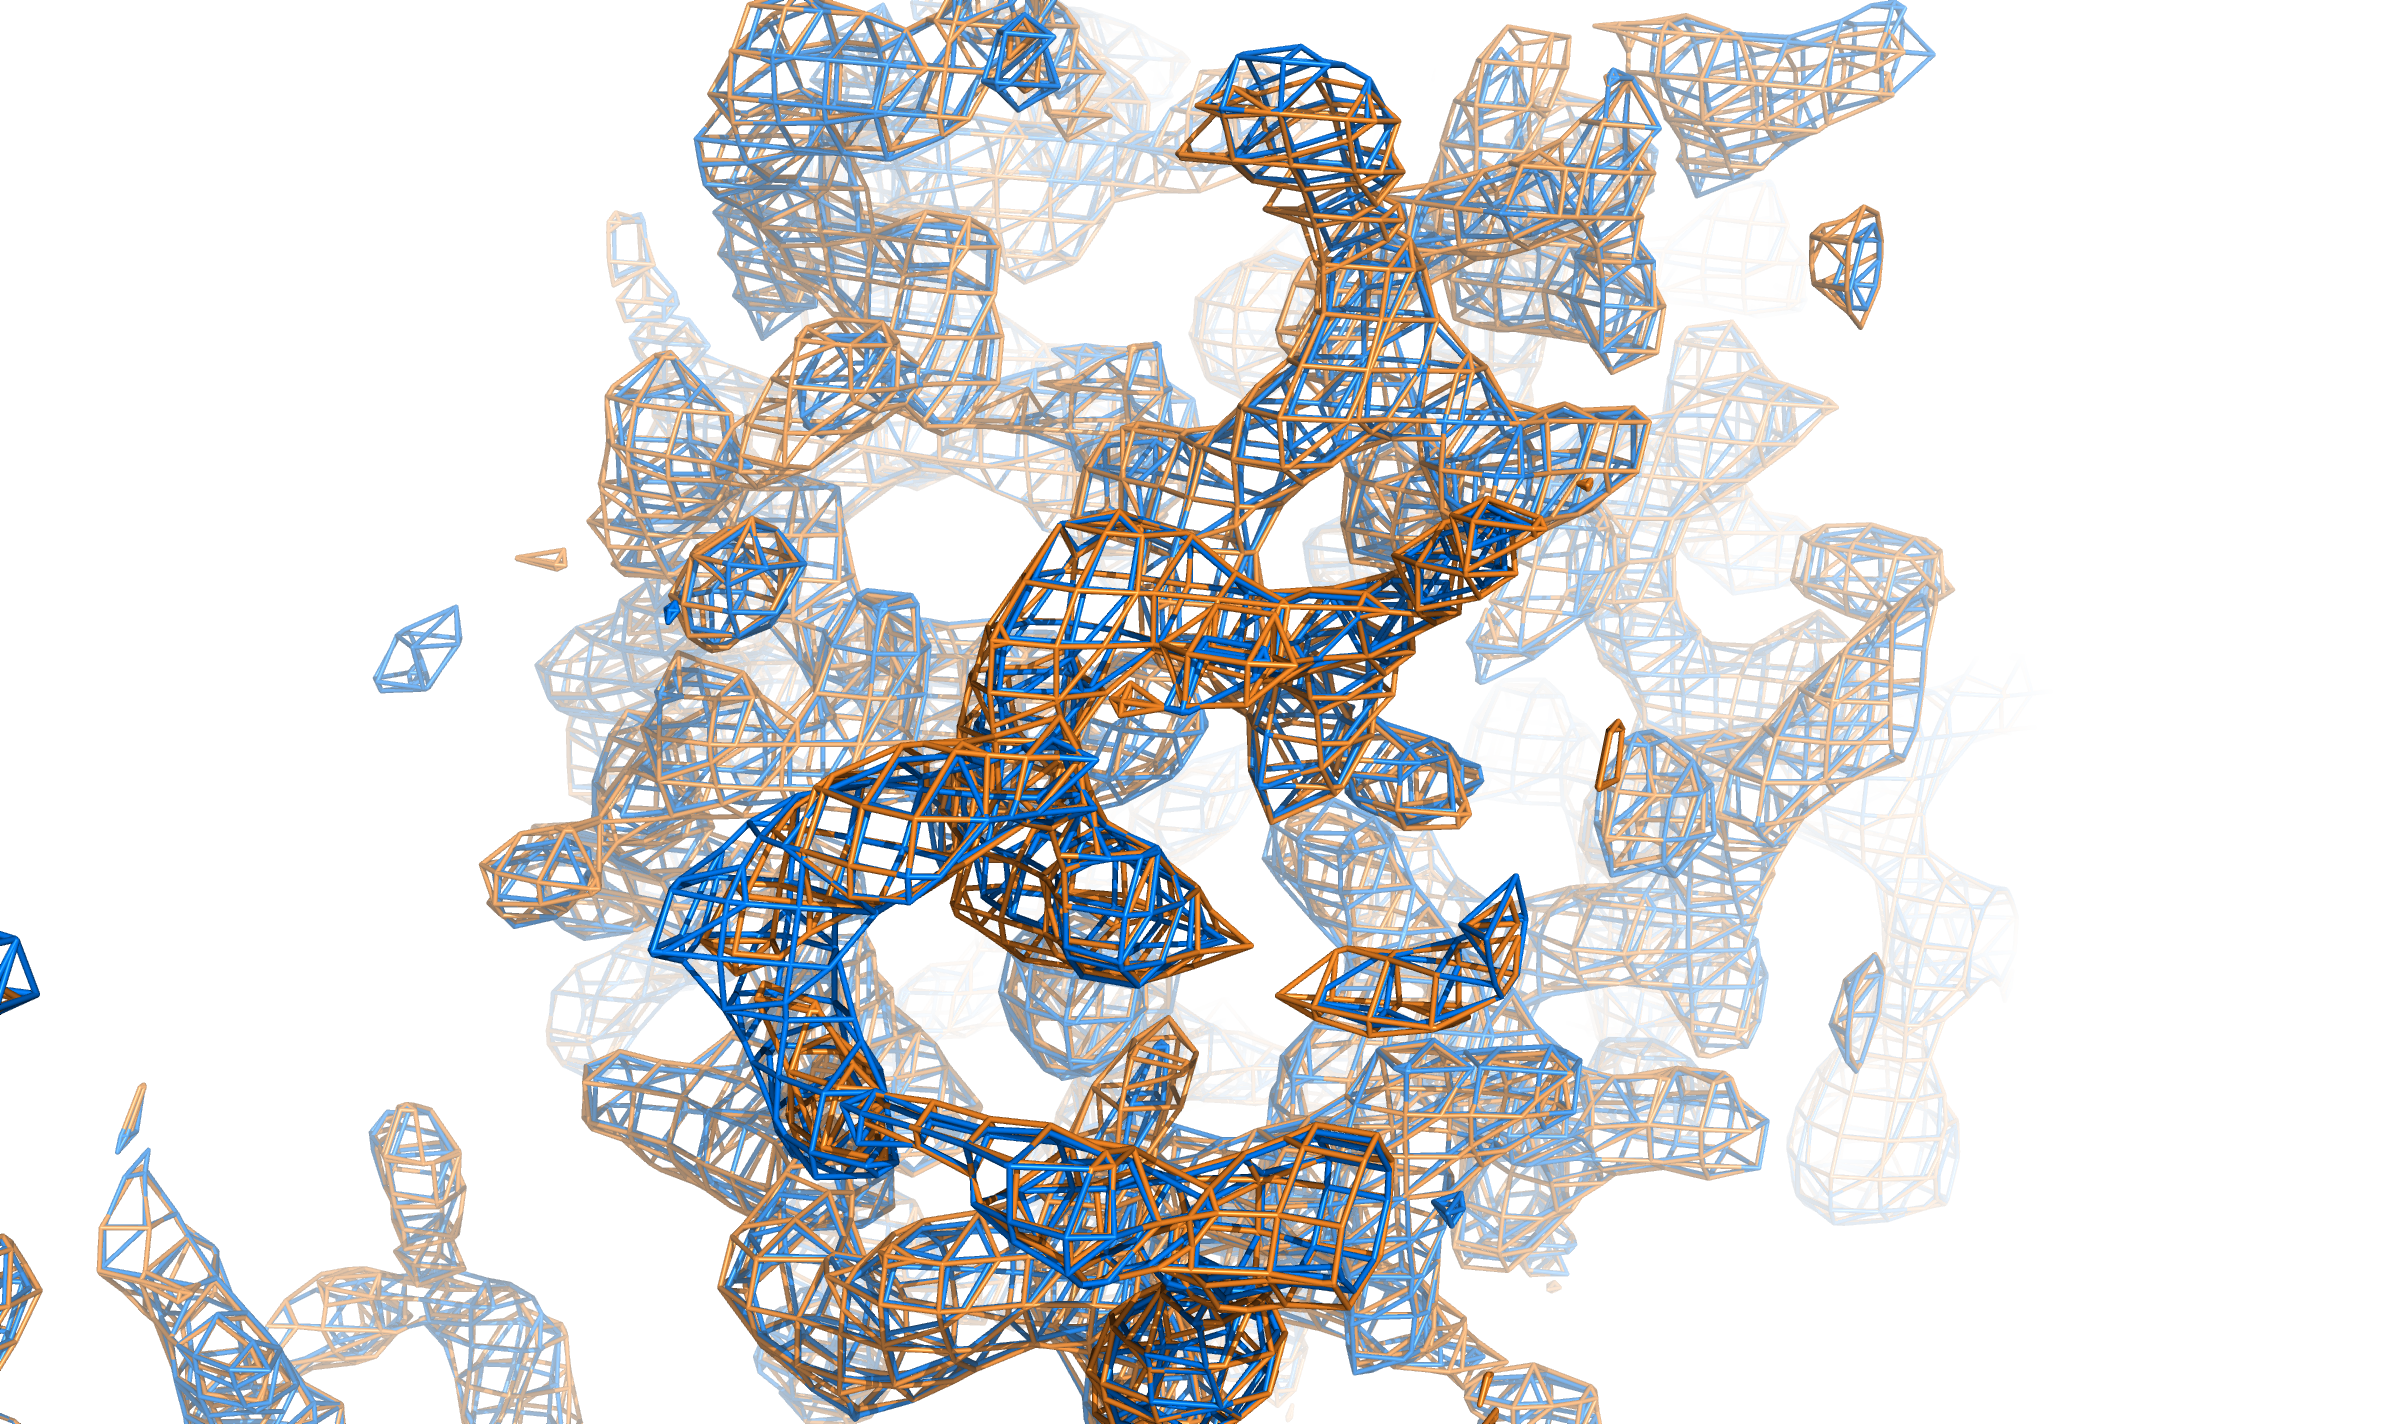
\includegraphics[width=\textwidth]{figures/datared/CPROT_elec_dens_comp2.png}
            \caption{}
            \label{fig:Electron density map 2 - C.Esp1396I}
    \end{subfigure}
    \caption{2F$_{\text{o}}$ - F$_{\text{c}}$ electron density maps contoured at the 3$\sigma$ level for the ACT pipeline (blue) and the FBA pipeline (orange).
    The regions of electron density shown in both (a) and (b) are representative of the density throughout the unit cell and generally both maps agree.}
    \label{fig:Electron density maps - C.Esp1396I}
\end{figure}

The difference map between the amplitude values calculated from the ACT and FBA pipelines, using phases from the resulting model from refinement of the ACT data, is shown in Figure~\ref{fig:Difference electron density map - C.Esp1396I}.
The difference density is no longer random and in fact is located around where the model is located in the unit cell.
This suggests that the two different pipelines could lead to different structural models.
\begin{figure}[ht!]
    \centering
    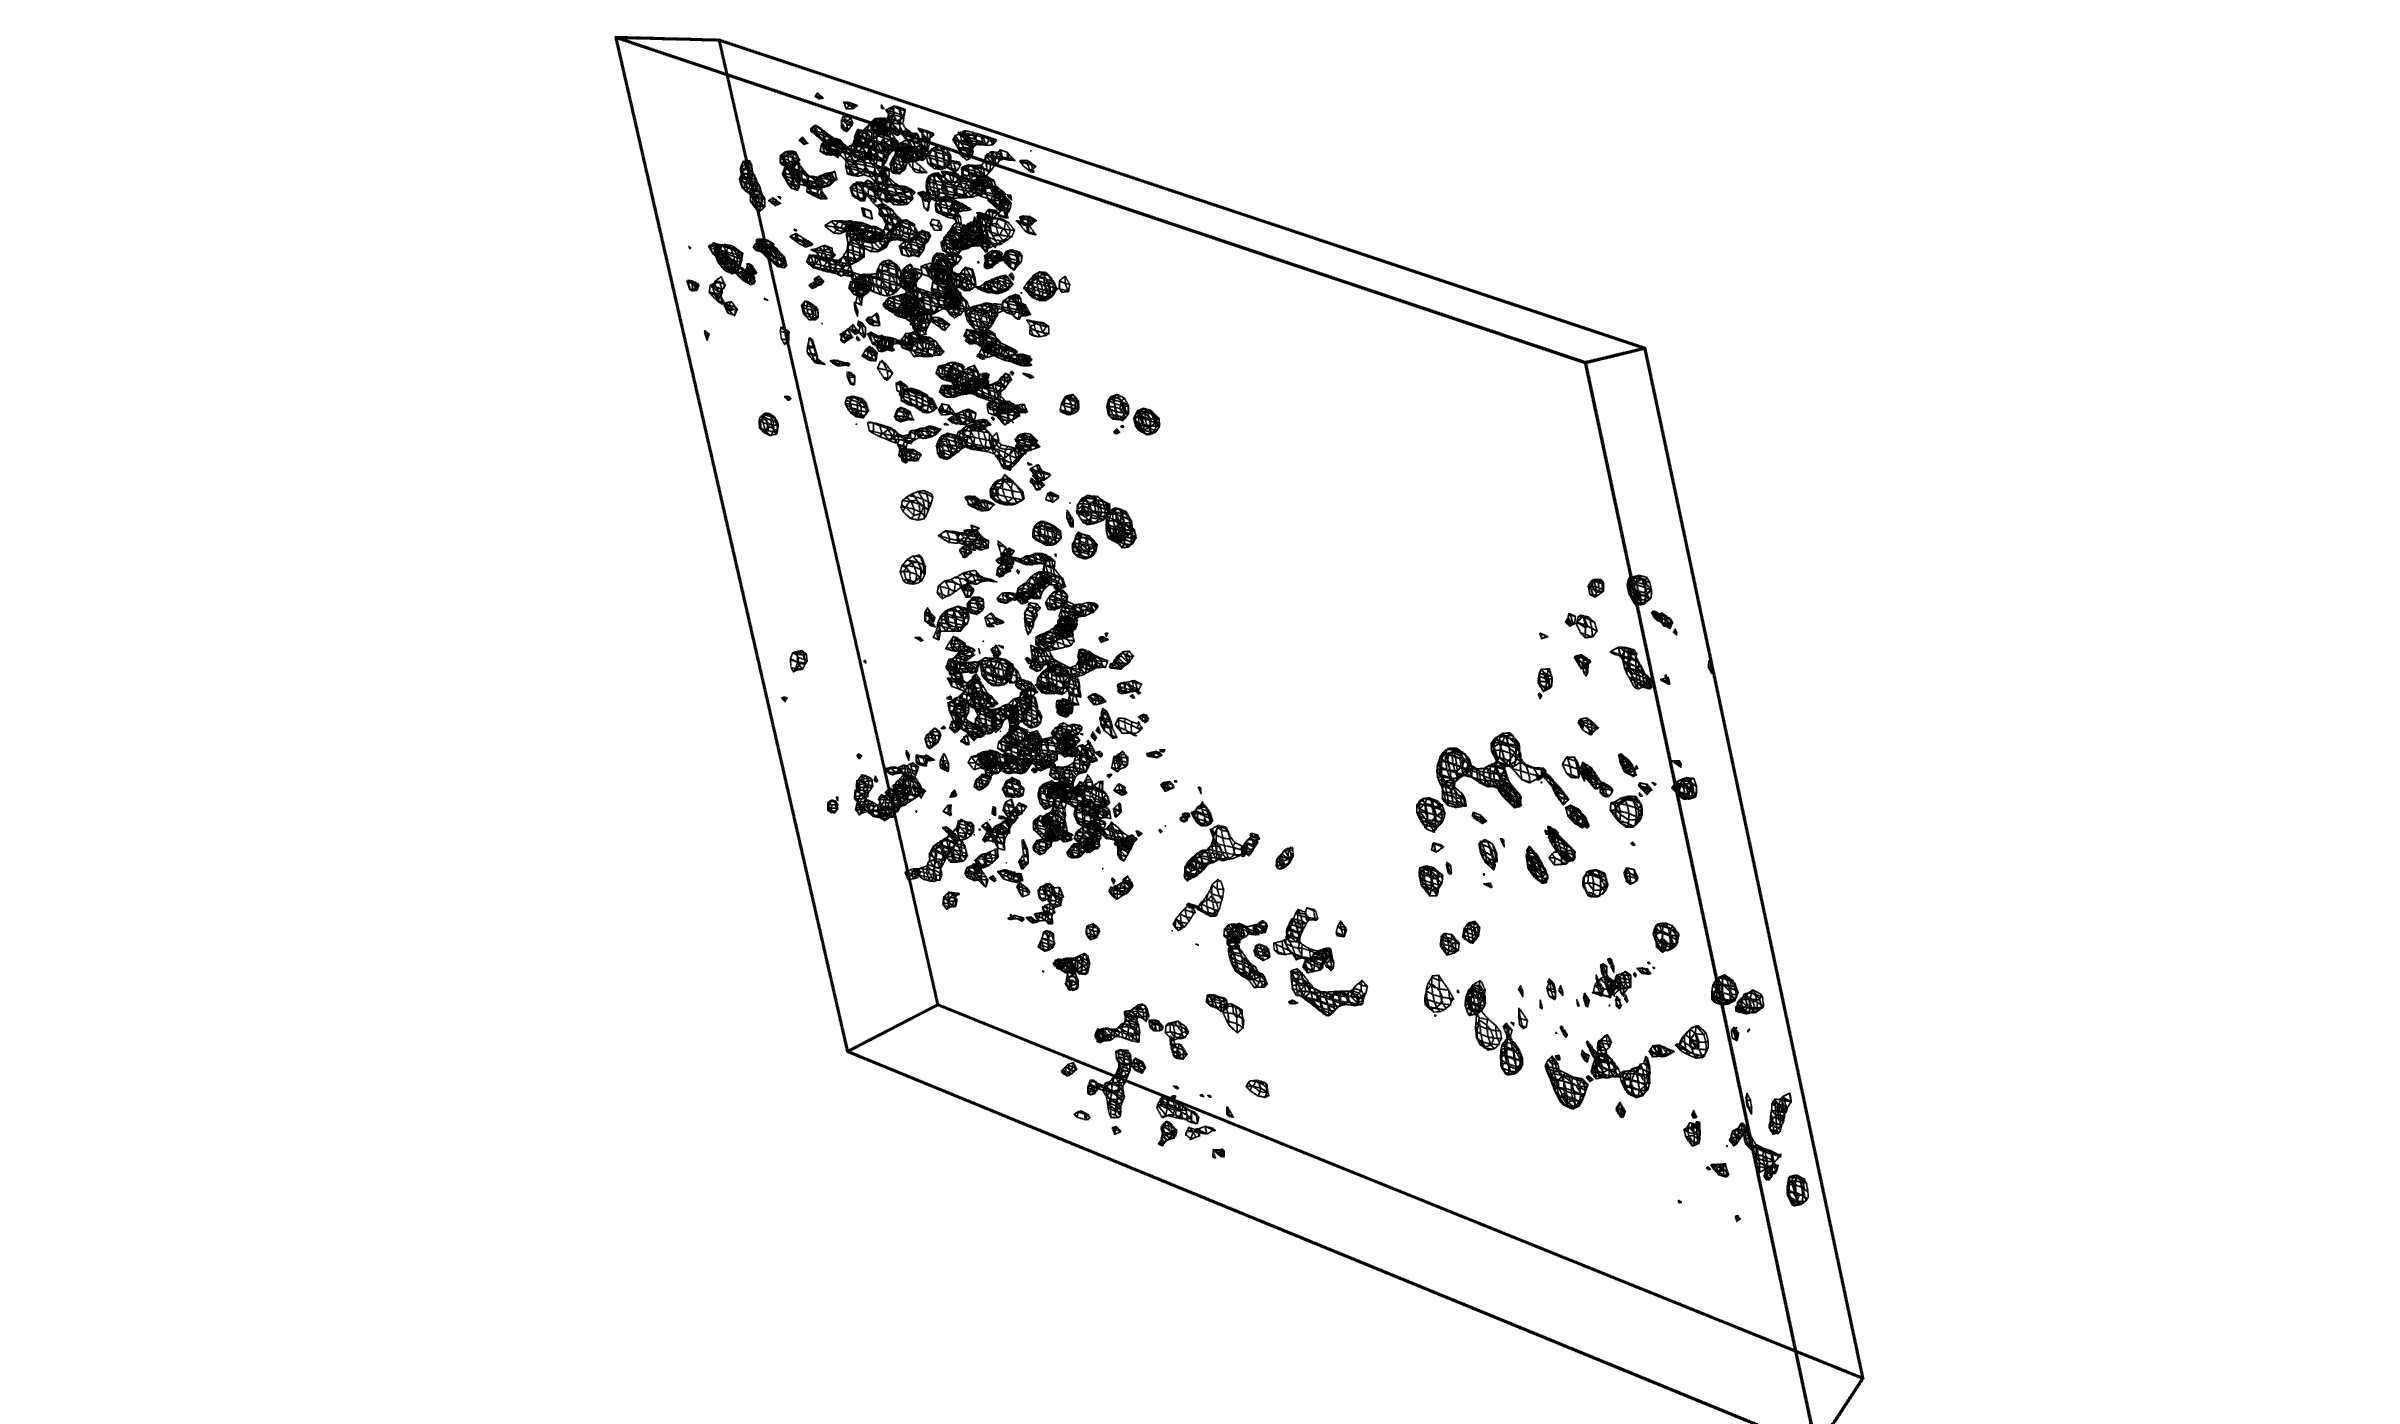
\includegraphics[width=1.0\textwidth]{figures/datared/CPROT_diff_map.png}
    \caption{Difference electron density map (black mesh) contoured at the 3$\sigma$ level between the amplitudes resulting from the ACT pipeline and the FBA pipeline using the phases obtained from the model resulting from refinement with the data processed using the ACT pipeline.
    The difference density is not random like it was for the insulin structure.
    Instead most of the difference density is located around the structure, suggesting that the refined models are likely to differ in several regions.}
    \label{fig:Difference electron density map - C.Esp1396I}
\end{figure}

Again the total number of reflections differ between datasets.
The FBA pipeline results in 32944 reflections at the end of data reduction, whereas the ACT pipeline results in 32898 reflections.

Overall refinement statistics using both pipelines are shown in Table \ref{tab:Refinement statistics - C.Esp1396I}.
The R values are slightly better for the ACT pipeline but the RMS values are lower for the FBA pipeline.
The statistics obtained using the FBA method are much better than expected considering the scale factor used in the FBA was incorrect.
If the amplitude values resulting from the FBA pipeline are indeed incorrect then it is likely that the refinement process is significantly``mopping up" the errors that are made during the data reduction stage.
It is also possible that the statistical improvement by manually refining the model may be more limited with the data for the FBA pipeline compared to that of the ACT pipeline.
\begin{table}[ht!]
	\caption{Final refinement statistics for data processed with the ACT and FBA pipelines}
	\centering
	\begin{tabular}{p{4cm} | p{2.5cm} | p{2.5cm}}
		   & ACT & FBA  \\
		\hline
		R work                      & 0.257   & 0.259 \\
		R free                      & 0.282   & 0.288 \\
		RMS bond length (\AA)       & 0.014   & 0.012 \\
        RMS Bond Angle ($^{\circ}$) & 1.937   & 1.806 \\
		\hline
	\end{tabular}
	\label{tab:Refinement statistics - C.Esp1396I}
\end{table}
